% =====================================================================
%  CERA-CPD: conformal sequential detection, retrospective delineation and
%  burden uncertainty for paroxysmal atrial fibrillation in ambulatory ECG.
%  Format: Elsevier numbered-reference template (elsarticle, preprint).
%  Figures in figures/, generated tables in tables/;
%  both are produced by experiments/cera_exp (aggregate.py, tables.py, figures.py).
% =====================================================================
\documentclass[preprint,12pt]{elsarticle}

\usepackage[T1]{fontenc}
\usepackage{amsmath,amssymb,amsfonts}
\usepackage{bm}
\usepackage{graphicx}
\usepackage{booktabs}
\usepackage{caption}
\usepackage{multirow}
\usepackage{array}
\usepackage{xcolor}
\usepackage{algorithm}
\usepackage{algpseudocode}
\usepackage{tikz}
\usetikzlibrary{arrows.meta,positioning,fit,calc,shapes.geometric,backgrounds}
\biboptions{numbers,sort&compress}
\usepackage{url}
\usepackage[hidelinks]{hyperref}
\hypersetup{pdfauthor={Muktesh Gupta, Pranjal Kumar, Himanshu Verma}}
% Allow flexible line breaking at the template's single-column width.
\setlength{\emergencystretch}{3em}
% Float placement: let floats share pages with text instead of leaving half-empty float pages.
\renewcommand{\topfraction}{0.9}
\renewcommand{\bottomfraction}{0.8}
\renewcommand{\textfraction}{0.07}
\renewcommand{\floatpagefraction}{0.8}
\renewcommand{\dbltopfraction}{0.9}
\renewcommand{\dblfloatpagefraction}{0.8}
\setcounter{topnumber}{3}
\setcounter{bottomnumber}{2}
\setcounter{totalnumber}{5}
\setcounter{dbltopnumber}{3}
\setlength{\floatsep}{10pt plus 2pt minus 2pt}
\setlength{\textfloatsep}{12pt plus 2pt minus 2pt}
\setlength{\intextsep}{10pt plus 2pt minus 2pt}
% Punctuation style: no colons after caption labels, keyword title, email note or algorithm headers.
\captionsetup{labelsep=period}
\keywordtitlesep{.\ }
\usepackage{etoolbox}
\makeatletter
\patchcmd{\printFirstPageNotes}{\textit{Email address:\space}}{\textit{Email address\space}}{}{}
\makeatother
\algrenewcommand\algorithmicrequire{\textbf{Input}}
\algrenewcommand\algorithmicensure{\textbf{Output}}
\algrenewcommand\alglinenumber[1]{\footnotesize #1}

% ---------------- macros ----------------
\newsavebox{\tablebox}
\newcommand{\fitwidth}[1]{%
  \sbox{\tablebox}{#1}%
  \ifdim\wd\tablebox>\linewidth
    \resizebox{\linewidth}{!}{\usebox{\tablebox}}%
  \else
    \usebox{\tablebox}%
  \fi}
\newcommand{\method}{CERA-CPD}
\newcommand{\E}{\mathbb{E}}
\newcommand{\Prob}{\mathbb{P}}
\newcommand{\1}{\mathbf{1}}
\DeclareMathOperator*{\argmax}{arg\,max}
\DeclareMathOperator*{\median}{median}


\hyphenation{elec-tro-car-dio-gram fib-ril-la-tion}

\begin{document}

\begin{frontmatter}

\title{Conformal Certification of Sequential Detectors for Paroxysmal Atrial Fibrillation Delineation and Burden Estimation in Ambulatory ECG}

\author[nitj]{Muktesh Gupta\corref{cor1}}
\ead{guptam@nitj.ac.in}
\author[nitj]{Pranjal Kumar}
\author[nitj]{Himanshu Verma}

\cortext[cor1]{Corresponding author.}

\affiliation[nitj]{organization={Department of Computer Science and Engineering, Dr. B. R. Ambedkar National Institute of Technology Jalandhar},
                  city={Jalandhar},
                  postcode={144008},
                  state={Punjab},
                  country={India}}

% =====================================================================
\begin{abstract}
Reliable delineation of paroxysmal atrial fibrillation (AF) remains challenging in ambulatory electrocardiogram monitoring. Missed or delayed boundaries distort AF burden, while false detections increase review workload. This motivates combining accurate episode timing, controlled alarm rates and uncertainty estimates despite noise, ectopy and patient variability. Classifiers and segmentation networks improve AF recognition and boundary prediction, but do not establish false-alarm budgets for new patients or quantify uncertainty from unobserved ECG. Sequential detection trades calibration against delay. This research proposes \method{}, integrating complementary rhythm representations, patient-adaptive conformal e-detection and uncertainty-aware burden estimation. A dual-stream encoder combines RR irregularity with QRST-residual atrial activity through quality- and rate-aware fusion and ectopy-aware contrastive training. Decision-clipped scores become conformal e-values against the wearer's history, accumulated for two-sided detection separating alarm issuance from retrospective beat-level localisation. A conformal gate certifies other sequential detectors' alarms under stated null conditions, while patient-level burden intervals account for quality-rejected time. Evaluation uses nested patient-wise cross-validation, independent cohorts, noise stress and end-to-end QRS detection. Under 0\,dB electrode-motion noise, the standalone detector produced 0.07 false episodes/h versus 0.31 for CUSUM, although short reference histories delayed detection. In secondary analyses, gating CUSUM reduced false episodes from 0.085 to 0.069/h ($p=0.004$) while retaining 95\% of its score, and wearer memory raised AFDB episode F1 from 16\% to 59\%. Nominal 90\% burden intervals achieved 93 to 97\% coverage in cross-validation and 94.4\% on AFDB (CUSUM). These findings favour conformal evidence as a certificate on conventional sequential detectors for limiting false alarms in long-term ambulatory monitoring.
\end{abstract}

\begin{keyword}
Atrial fibrillation \sep change-point detection \sep conformal prediction \sep e-values \sep wearable electrocardiography \sep AF burden
\end{keyword}

\end{frontmatter}

% =====================================================================
\section{Introduction}
\label{sec:intro}

Atrial fibrillation (AF) is the most common sustained arrhythmia and a major cause of stroke, heart failure and hospitalisation \cite{vangelder2024esc}. Because time spent in AF is associated with the risk of ischaemic stroke \cite{becher2024burden}, AF is characterised by its burden as well as its presence \cite{becher2024burden,vangelder2024esc}. Continuous monitoring with Holter recorders, patches and smartwatches \cite{mannhart2023basel,aguilar2025smartwatch} supports such assessment only if each onset and offset is located accurately, since missed or delayed boundaries distort AF duration, while false episodes inflate burden and the clinical review workload. The 4th China Physiological Signal Challenge (CPSC2021) made this delineation task explicit by scoring onsets and offsets at beat resolution \cite{cpsc2021}, although its short annotated events are a signal-processing target rather than a clinical diagnosis.

Delineation is an online change-point detection (CPD) problem with alternating onset and offset events \cite{gupta2024review}, complicated by noise and by ectopic beats, sinus arrhythmia and atrial flutter, which mimic the RR irregularity of AF \cite{cpsc2021}. Rhythm-based detectors use RR-transition Markov models \cite{moody1983afdb,kalidas2019markov}, coefficients of variation \cite{tateno2001} or COSEn \cite{lake2011cosen}. Waveform approaches add atrial information through QRST cancellation \cite{stridh2001qrst} and f-wave changes \cite{petrutiu2007ltafdb}. Deep networks learn from RR sequences \cite{faust2018}, raw ECG \cite{salvi2024aiaf} and contrastive representations across patients \cite{kiyasseh2021clocs}, and U-Net-based event detectors \cite{wen2022paf}, a self-supervised Transformer \cite{yun2024safer} and AF-DETR \cite{wang2025afdetr} estimate beat-level labels on CPSC2021. Boundary prediction alone, however, neither establishes a false-alarm budget for a new wearer nor quantifies uncertainty in the accumulated AF time.

Sequential CPD connects accumulated evidence to alarm control. The cumulative sum (CUSUM) procedure \cite{page1954} and the Shiryaev and Roberts (SR) procedure \cite{shiryaev1963,roberts1966} use pre- and post-change models, and Bayesian online CPD \cite{adams2007bocpd}, density-ratio estimation \cite{liu2013rulsif} and learned contrastive representations \cite{deldari2021tscp2} relax these assumptions, but development-set thresholds do not guarantee an alarm rate on a new patient \cite{gupta2024review}. Conformal methods provide such guarantees under stated conditions. Online conformal p-values are independent and uniform for exchangeable scores \cite{vovk2003testing,vovk2022alrw}, supporting conformal change detectors \cite{volkhonskiy2017icm,vovk2025cusum}. Calibrators turn p-values into e-values \cite{vovk2021evalues}, which support anytime-valid inference \cite{ramdas2023savi} and e-detectors with average-run-length control \cite{shin2024edetectors}, and split conformal prediction supplies finite-sample marginal intervals \cite{lei2018split}. However, standard conformal martingales can incur suboptimal detection delay \cite{bhattacharyya2026conformal}.

This research proposes \method{} (Conformal E-detection of Rhythm and Atrial-activity changes), an online framework that turns a learned AF representation into a calibrated episode delineator. It aims to learn rhythm and atrial features that separate AF from irregular non-AF activity, to test whether conformal evidence can control alarm workload alone or as a certificate on a conventional detector, to localise boundaries at beat level using only data available at the alarm, and to estimate burden with intervals that account for unobserved time. The main contributions are as follows.

\begin{itemize}
\item A decision-clipped conformal e-detector that preserves null validity under exchangeable fixed-mode scores and separates alarm issuance from retrospective beat-level localisation.
\item A conformal certification gate through which alarms proposed by any sequential detector inherit a run-length bound under the stated null conditions, independently of the proposing detector's training.
\item A state-conditional wearer memory, with margin clipping and a resolution-matched calibrator that keep the e-values exact, so that conformal evidence draws on a wearer's earlier episodes and recordings.
\item A dual-stream representation of RR irregularity and QRST-residual atrial activity with quality- and rate-aware fusion and ectopy-aware supervised contrastive training.
\item Patient-level split-conformal burden intervals with a deterministic expansion for quality-rejected time.
\end{itemize}

The remainder of the manuscript is organised as follows. Section~\ref{sec:method} describes the proposed framework, Section~\ref{sec:setup} the hypotheses, datasets and evaluation protocol, and Section~\ref{sec:results} the results, including the secondary analyses. Section~\ref{sec:discussion} discusses the findings and limitations, and Section~\ref{sec:conclusion} concludes the manuscript.

% =====================================================================
\section{Proposed Method}
\label{sec:method}
A wearable AF delineator must be causal, control false alarms for each new wearer, place boundaries at beat level and report burden with its uncertainty, including time lost to noise. \method{} meets these requirements in three phases (Fig.~\ref{fig:overview}). Phase~I forms quality-checked blocks of beats with explicit release times, which gives causality and a common unit of evidence. Phase~II maps each block to a score of how strongly it contradicts the current rhythm state. Phase~III ranks this score against the wearer's own history, which controls false alarms without a population threshold, and then localises each change and bounds the burden. Because the decision rule is separate from the representation, the same encoder can be paired with other decision rules, which enables fair comparison and the certification variant of Section~\ref{sec:gate}.

% ---------------- Overview figure (TikZ, renders as-is) ----------------
\begin{figure*}[!htbp]
\centering
\resizebox{\textwidth}{!}{%
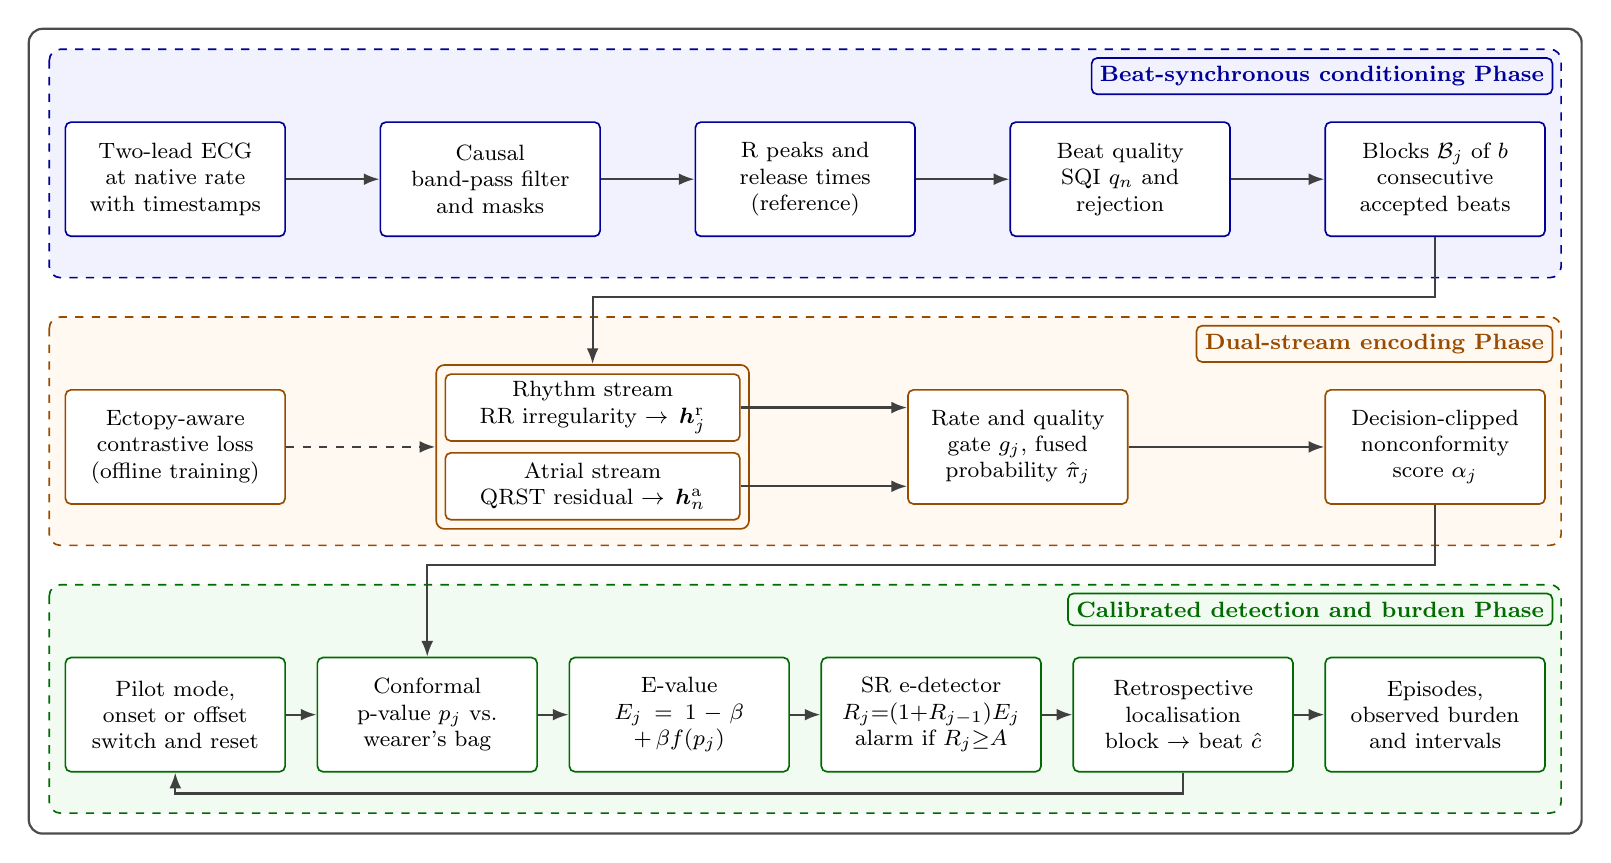
\begin{tikzpicture}[
  font=\footnotesize,
  box/.style={draw=#1!60!black, rounded corners=2pt, align=center, text width=2.65cm, minimum height=1.45cm, inner sep=2pt, fill=white, line width=0.6pt, execute at begin node={\hyphenpenalty=10000}},
  sbox/.style={draw=#1!60!black, rounded corners=2pt, align=center, text width=3.6cm, minimum height=0.85cm, inner sep=2pt, fill=white, line width=0.6pt},
  arr/.style={-{Latex[length=2mm]}, thick, draw=black!75},
  tab/.style={draw=#1!60!black, text=#1!60!black, font=\footnotesize\bfseries, rounded corners=2pt, line width=0.6pt, inner sep=3pt, anchor=north east}
]
% Grid: panels span x in [-1.6,17.6]; row centres at y = 0, -3.4, -6.8.
\colorlet{cI}{blue}\colorlet{cII}{orange}\colorlet{cIII}{green!70!black}
% ---- phase panels (drawn first, behind the boxes)
\foreach \y/\c in {0/cI, -3.4/cII, -6.8/cIII}
  \draw[draw=\c!60!black, dashed, rounded corners=4pt, fill=\c!5, line width=0.6pt] (-1.6,\y+1.65) rectangle (17.6,\y-1.25);
\node[tab=cI]   at (17.5,1.55)  {Beat-synchronous conditioning Phase};
\node[tab=cII]  at (17.5,-1.85) {Dual-stream encoding Phase};
\node[tab=cIII] at (17.5,-5.25) {Calibrated detection and burden Phase};
% ---- Phase I (left to right, five equally spaced steps)
\node[box=cI] (in)  at (0,0)  {Two-lead ECG\\at native rate\\with timestamps};
\node[box=cI] (bp)  at (4,0)  {Causal\\band-pass filter\\and masks};
\node[box=cI] (qrs) at (8,0)  {R peaks and\\release times\\(reference)};
\node[box=cI] (sqi) at (12,0) {Beat quality\\SQI $q_n$ and\\rejection};
\node[box=cI] (blk) at (16,0) {Blocks $\mathcal{B}_j$ of $b$\\consecutive\\accepted beats};
% ---- Phase II
\node[box=cII] (con) at (0,-3.4) {Ectopy-aware\\contrastive loss\\(offline training)};
\node[sbox=cII] (rr) at (5.3,-2.9) {Rhythm stream\\RR irregularity $\to\bm{h}^{\mathrm r}_j$};
\node[sbox=cII] (at) at (5.3,-3.9) {Atrial stream\\QRST residual $\to\bm{h}^{\mathrm a}_n$};
\node[draw=cII!60!black, rounded corners=3pt, inner sep=3pt, line width=0.6pt, fit=(rr)(at)] (enc) {};
\node[box=cII] (gate) at (10.7,-3.4) {Rate and quality\\gate $g_j$, fused\\probability $\hat\pi_j$};
\node[box=cII] (nc)   at (16,-3.4)   {Decision-clipped\\nonconformity\\score $\alpha_j$};
% ---- Phase III (six equally spaced steps)
\node[box=cIII] (mode) at (0,-6.8)    {Pilot mode,\\onset or offset\\switch and reset};
\node[box=cIII] (cp)   at (3.2,-6.8)  {Conformal\\p-value $p_j$ vs.\\wearer's bag};
\node[box=cIII] (ev)   at (6.4,-6.8)  {E-value\\$E_j=1-\beta$\\$+\,\beta f(p_j)$};
\node[box=cIII] (sr)   at (9.6,-6.8)  {SR e-detector\\$R_j{=}(1{+}R_{j-1})E_j$\\alarm if $R_j{\ge}A$};
\node[box=cIII] (loc)  at (12.8,-6.8) {Retrospective\\localisation\\block $\to$ beat $\hat c$};
\node[box=cIII] (out)  at (16,-6.8)   {Episodes,\\observed burden\\and intervals};
% ---- arrows within phases
\draw[arr] (in) -- (bp); \draw[arr] (bp) -- (qrs); \draw[arr] (qrs) -- (sqi); \draw[arr] (sqi) -- (blk);
\draw[arr, dashed] (con.east) -- (enc.west);
\draw[arr] (rr.east) -- (gate.west|-rr.east);
\draw[arr] (at.east) -- (gate.west|-at.east);
\draw[arr] (gate) -- (nc);
\draw[arr] (mode) -- (cp); \draw[arr] (cp) -- (ev); \draw[arr] (ev) -- (sr); \draw[arr] (sr) -- (loc); \draw[arr] (loc) -- (out);
\draw[arr] (loc.south) -- (12.8,-7.8) -| (mode.south);
% ---- arrows between phases (routed through the gaps between panels)
\draw[arr] (blk.south) -- (16,-1.5) -| (enc.north);
\draw[arr] (nc.south) -- (16,-4.9) -| (cp.north);
% ---- outer frame
\draw[black!70, line width=0.8pt, rounded corners=5pt]
  ([shift={(-0.25,-0.25)}]current bounding box.south west) rectangle ([shift={(0.25,0.25)}]current bounding box.north east);
\end{tikzpicture}}
\caption{Overview of \method{} with quality-gated eight-beat blocks (Phase~I), a frozen dual-stream encoder (Phase~II), and conformal e-detection with Shiryaev and Roberts accumulation, localisation and burden intervals (Phase~III). Dashed arrows denote offline training.}
\label{fig:overview}
\end{figure*}

% ---------------------------------------------------------------------
\subsection{Problem Formulation and Notation}
\label{sec:formulation}
A monitored ECG is a stream $\bm{x}_t\in\mathbb{R}^{2}$ of two leads at native sampling frequency $f_s$, whose timestamps are retained. Let $r_n$ be the time of confirmed R peak $n$, $\mathrm{RR}_n=r_n-r_{n-1}$, and $s_n\in\{0,1\}$ the annotated rhythm, with AF and atrial flutter merged as in the challenge. For episode $e$, $c_e^+$ is the first AF beat and $c_e^-$ the first subsequent non-AF beat. Episodes are half-open intervals $[a_e,d_e)$ with $a_e=r_{c_e^+}$ and $d_e=r_{c_e^-}$, and endpoints at the recording boundaries are censored. Burden is elapsed time rather than the proportion of AF beats, which would overstate it because AF usually has a higher ventricular rate,
\begin{equation}
B=\frac{\left|\bigcup_e[a_e,d_e)\right|}{T},
\label{eq:burden}
\end{equation}
where $|\cdot|$ denotes duration and $T$ the recording duration. The online delineator watches for an onset in mode $m=0$ and for an offset in mode $m=1$, and each alarm is paired with a retrospective boundary estimate $\hat c$ computed from data available at the alarm. Algorithm~\ref{alg:cera} summarises the operation and Table~\ref{tab:notation} the notation.

\begin{table}[!htbp]
\centering
\caption{Main notation.}
\label{tab:notation}
\footnotesize
\setlength{\tabcolsep}{3pt}
\fitwidth{%
\begin{tabular}{@{}>{\raggedright\arraybackslash}p{1.6cm}>{\raggedright\arraybackslash}p{4.7cm}>{\raggedright\arraybackslash}p{1.6cm}>{\raggedright\arraybackslash}p{4.7cm}@{}}
\toprule
Symbol & Meaning & Symbol & Meaning \\
\midrule
$f_s$, $L$ & native sampling frequency, waveform grid length ($L=64$ samples) & $\alpha_j$ & mode-dependent nonconformity score of block $j$ \\
$r_n, \mathrm{RR}_n$ & time of R peak $n$, RR interval ending at beat $n$ & $p_j$, $\theta_j$ & online smoothed conformal p-value, tie-breaking uniform \\
$s_n$, $m$ & rhythm state of beat $n$ (1 = AF), detector mode & $f$, $E_j$, $\beta$ & calibrator, e-value, betting fraction \\
$c^{+}, c^{-}, \hat c$ & true onset, true offset, estimated boundary beat & $R_j$, $A$, $\tau$ & Shiryaev and Roberts statistic, alarm threshold, alarm block \\
$q_n, q_{\min}$ & beat quality index and abstention threshold & $W$ & warm-up blocks after every reset \\
$b$, $\mathcal{B}_j$ & block size (beats) and $j$-th block of accepted beats & $\eta$, $u$ & localisation tolerance, heuristic localisation spread (beats) \\
$\bm{h}^{\mathrm r}_j$, $\bm{h}^{\mathrm a}_n$ & rhythm-stream (block) and atrial-stream (beat) embeddings & $\omega$ & localisation-based scale for burden residuals \\
$\pi^{\mathrm r}_j, \pi^{\mathrm a}_j, \hat\pi_j$ & stream-wise and fused block AF probabilities & $\delta_{\mathrm R}$, $\delta$ & nominal R-peak latency (0.15\,s), burden miscoverage level (0.1) \\
$\pi_n$, $g_j$ & beat-level AF probability (localisation), rate- and quality-aware fusion gate & $\hat B_o$, $C^o_{1-\delta}$ & estimated observed-time AF burden and its conformal interval \\
\bottomrule
\end{tabular}}
\end{table}


% ---------------------------------------------------------------------
\subsection{Beat-Synchronous Conditioning (Phase I)}
\label{sec:phase1}
\subsubsection{Filtering and R peaks}
Each lead is filtered at its native rate by a fourth-order causal Butterworth band-pass (0.5 to 40\,Hz, second-order sections), which suppresses baseline wander and high-frequency noise without future samples. The main experiments use the reference beat annotations as R peaks. This \emph{reference-peak track} isolates the encoder and detector from QRS-detection errors, whose effect is evaluated separately with a causal detector of the Pan and Tompkins type \cite{pan1985} (Section~\ref{sec:protocol}).

\subsubsection{Beat quality}
Noisy beats create spurious irregularity and must be rejected, whereas ectopic beats must be kept so that the detector learns to tolerate them. A kurtosis index \cite{li2008sqi} rejected 365 of 468 premature ventricular beats in a development recording, so a detector-agreement criterion \cite{li2008sqi,behar2013sqi} is used instead. It requires a clean beat cell to contain no QRS-like energy other than its own complex, which ectopic beats satisfy and noise bursts usually violate. With the slope-energy envelope $e(t)$ of a lead (squared first difference, 100-ms moving average),
\begin{equation}
\rho_n=\frac{\max_{t\in[r_n+0.3,\;r_{n+1}-0.15]}e(t)}{\max_{|t-r_n|\le0.1}e(t)},
\label{eq:sqi}
\end{equation}
and $q_n=\max_{\text{leads}}\min\{1,\max\{0,(0.7-\rho_n)/0.4\}\}$, set to zero for flat (s.d.\ $<5\,\mu$V) or saturated ($>10$\,mV peak-to-peak) windows $[r_n-0.3,r_n+0.5)$\,s. A beat with $q_n<q_{\min}=0.5$ is rejected.

\subsubsection{Beat blocks}
AF is recognised from the irregularity of several successive RR intervals, so accepted beats are grouped into blocks, the unit of all later scoring. A complete block contains $b=8$ consecutive accepted beats with internal RR intervals in $[0.2,3]$\,s and a confirmed next peak, which balances evidence per block against time resolution (sizes 4 and 16 are examined in Section~\ref{sec:res-ablation}). Its rhythm input is the $b-1$ internal intervals divided by their median, which removes the heart rate so that the encoder sees irregularity alone. Blocks do not overlap, so successive scores never share beats. A rejected beat or an out-of-range interval discards the pending partial block, which then contributes neither evidence nor observed time. Unobserved stretches shorter than $G=30$\,s only remove blocks, whereas a longer stretch resets the detector (Section~\ref{sec:phase3}).

The waveform input of a block beginning at $r_\ell$ is restricted to $[r_\ell,r_{\ell+b})$, so that no information leaks between blocks. Per beat, the pre-QRS interval $[-\min(0.4,0.7\mathrm{RR}_n),-0.06]$\,s, where P waves or f-waves appear, and an R-aligned $[-0.25,0.45]$\,s interval are interpolated onto $L=64$ points, with samples outside the support masked. QRST residuals subtract the sample-wise masked median of the aligned windows of the block \cite{stridh2001qrst}, which cancels the ventricular complex and exposes atrial activity, and each lead is normalised by the median and median absolute deviation of its supported samples. To keep every decision causal, a block is released only at $a_j=\max\{r_{\ell+b}+\delta_{\mathrm R},\,r_{\ell+b-1}+0.5\,\mathrm{s}\}$, with a nominal R-peak confirmation latency $\delta_{\mathrm R}=0.15$\,s, when the quality window of its final beat is complete.

% ---------------------------------------------------------------------
\subsection{Dual-Stream Encoding and Nonconformity (Phase II)}
\label{sec:phase2}
Phase~II condenses each block into one nonconformity score for Phase~III to rank. RR irregularity is the most robust AF marker but is mimicked by ectopy, whereas atrial activity separates AF from irregular non-AF rhythms but fails at high ventricular rates and in noise. Each source therefore has its own stream, and a learned gate decides how far to trust each. The encoder is trained offline and then frozen, which keeps the score a fixed function of the block, as the conformal guarantees require.

\subsubsection{Rhythm and atrial streams}
The rhythm stream is a three-layer one-dimensional convolutional encoder (kernel sizes 7, 5 and 3, GELU, dropout, temporal mean pooling). Its output is concatenated with five descriptors that encode established AF markers, namely the log median internal RR, which restores the rate removed by median normalisation, the median-normalised RMSSD, the coefficient of variation, the turning-point ratio and a regularised sample entropy $-\log[(N_3+1)/(N_2+1)]$ of length-three RR subsequences at tolerance $0.2\,\mathrm{SD}(\Delta)$ \cite{richman2000sampen}, which is related to but not a reproduction of COSEn \cite{lake2011cosen}. A linear GELU layer yields $\bm h^{\mathrm r}_j\in\mathbb R^d$. The atrial stream is a separate encoder with the same kernel sizes, applied to each beat with four masked channels, the pre-QRS windows and the QRST residuals of both leads. Invalid values are zeroed after every layer and excluded from pooling, giving beat embeddings $\bm h^{\mathrm a}_n\in\mathbb R^d$ and their valid-beat average $\bar{\bm h}^{\mathrm a}_j$. No batch normalisation is used, so a block's output never depends on other blocks in a batch.

\subsubsection{Fusion and output heads}
Each stream has a block-level AF probability head, $\pi^{\mathrm r}_j=\sigma(\bm{w}_{\mathrm r}^{\top}\bm{h}^{\mathrm r}_j+b_{\mathrm r})$ and $\pi^{\mathrm a}_j=\sigma(\bm{w}_{\mathrm a}^{\top}\bar{\bm{h}}^{\mathrm a}_j+b_{\mathrm a})$. The two are fused in the logit domain by a gate $g_j\in[0,1]$,
\begin{equation}
\begin{aligned}
\hat\pi_j&=\sigma\!\bigl(g_j\,\mathrm{logit}\,\pi^{\mathrm r}_j+(1-g_j)\,\mathrm{logit}\,\pi^{\mathrm a}_j\bigr),\\
g_j&=\sigma\bigl(\phi(\bar q_j,\,\log\widetilde{\mathrm{RR}}_j)\bigr),
\end{aligned}
\label{eq:fusion}
\end{equation}
where $\phi$ is a two-layer perceptron of the mean beat quality $\bar q_j$ and the log median RR interval $\widetilde{\mathrm{RR}}_j$. The gate sees quality and rate because these are the conditions under which the atrial stream fails, so weight can shift to the rhythm stream. Since block outputs cannot resolve a boundary within a block, a beat-level head $\pi_n=\sigma(\bm{w}_{\mathrm b}^{\top}[\bm{h}^{\mathrm a}_n,\bm{h}^{\mathrm r}_j]+b_{\mathrm b})$ combines the atrial embedding of each beat with the rhythm context of its block and serves localisation (Section~\ref{sec:localisation}).

\subsubsection{Ectopy-aware supervised contrastive training}
Block labels alone do not teach the encoder that ectopic irregularity is not AF, nor that blocks of one patient can differ in rhythm. The encoders, heads and gate are therefore trained on training patients with a contrastive term added to the classification losses,
\begin{equation}
\mathcal{L}=\mathcal{L}_{\mathrm{bce}}(\hat\pi)+\lambda_{\mathrm s}\bigl[\mathcal{L}_{\mathrm{bce}}(\pi^{\mathrm r})+\mathcal{L}_{\mathrm{bce}}(\pi^{\mathrm a})\bigr]+\lambda_{\mathrm b}\mathcal{L}_{\mathrm{bce}}(\pi_n)+\lambda_{\mathrm c}\mathcal{L}_{\mathrm{con}}.
\label{eq:loss}
\end{equation}
The stream-wise terms keep each stream informative on its own, so the gate always has two usable inputs, and $\mathcal{L}_{\mathrm{con}}$ is a supervised contrastive loss \cite{khosla2020supcon} on $\ell_2$-normalised projections $\bm{z}_j$ of the concatenated block embeddings,
\begin{equation}
\mathcal{L}_{\mathrm{con}}=-\frac{1}{|\mathcal I_+|}\sum_{i\in\mathcal I_+}\frac{1}{|P(i)|}\sum_{p\in P(i)}\log\frac{\exp(\bm{z}_i^{\top}\bm{z}_p/\kappa)}{\sum_{a\in\mathcal{I}\setminus\{i\}}\exp(\bm{z}_i^{\top}\bm{z}_a/\kappa)},
\label{eq:supcon}
\end{equation}
with temperature $\kappa$, positives $P(i)$ defined by the block label (at least half of its beats AF) and $\mathcal I_+=\{i\in\mathcal I\mid|P(i)|>0\}$. The batch composition targets the two nuisances. Half of each batch of 256 blocks is drawn uniformly, a quarter are \emph{ectopy-nuisance positives}, non-AF blocks with at least one annotated ectopic beat (A, a, J, S, V, F or E), which place ectopy with sinus rhythm, and a quarter are \emph{patient-matched negatives}, opposite-rhythm blocks of the same patient as uniform anchors, which make the loss separate rhythm rather than patient identity. Beat BCE uses only beats with valid support. Augmentation mimics recording variability, with log-normal amplitude scaling (s.d.\ 0.25), Gaussian noise (s.d.\ 0.1), a random lead swap and a shift of up to two grid samples for the waveforms and log-normal jitter (s.d.\ 0.02) for the RR intervals.

\subsubsection{Decision-clipped nonconformity score}
In mode $0$ a block is nonconforming if it looks like AF, and in mode $1$ if it does not. Ranking the raw $\hat\pi_j$ would make the detector respond to \emph{any} departure from the wearer's history, such as a burst of ectopy that moves $\hat\pi_j$ from 0.01 to 0.3 without crossing the decision boundary, and such departures would accumulate into false alarms. The score is therefore clipped at the decision boundary,
\begin{equation}
\alpha_j=\begin{cases}\max\{\hat\pi_j,\tfrac12\}, & m=0,\\ \max\{1-\hat\pi_j,\tfrac12\}, & m=1,\end{cases}
\label{eq:nonconf}
\end{equation}
implemented as $\max\{\pm\ell_j,0\}$ on the fused logit $\ell_j$. All blocks consistent with the current state are then tied, and only blocks on the other side of the boundary count as evidence. Because \eqref{eq:fusion} depends only on the block and all parameters are fixed after training, $\alpha_j$ remains a fixed function of the block, and with the randomised tie-breaking of \eqref{eq:pvalue} fixed-mode rank validity is preserved \cite{vovk2022alrw}.

% ---------------------------------------------------------------------
\subsection{Calibrated Two-Sided Detection (Phase III)}
\label{sec:phase3}
A fixed threshold on $\hat\pi_j$ cannot control the false-alarm rate of a new wearer, because score distributions differ between patients and recording conditions. Phase~III therefore ranks each block against the wearer's own blocks since the last detected change. The ranks give conformal p-values valid for any score distribution, a calibrator turns them into e-values that can be multiplied over time, and the Shiryaev and Roberts recursion accumulates these into a statistic whose threshold sets the alarm budget. After an alarm, the boundary is located retrospectively and the mode switches.

\subsubsection{Online conformal p-values}
Let $\mathcal S$ be the reference bag of scores since the most recent reset, whose first block is block $1$. For block $j$, the smoothed conformal p-value is
\begin{equation}
p_j=\frac{\bigl|\{i\le j\mid\alpha_i>\alpha_j\}\bigr|+\theta_j\,\bigl|\{i\le j\mid\alpha_i=\alpha_j\}\bigr|}{j},
\label{eq:pvalue}
\end{equation}
with $\theta_j$ independent and uniform on $[0,1]$, which breaks the ties created by clipping without biasing the p-value. A small $p_j$ means that block $j$ is more AF-like (mode~0) or less AF-like (mode~1) than nearly all of the wearer's blocks in the current segment. If the scores of a change-free segment are exchangeable, which requires the initial mode to be selected independently of them and all parameters to be fixed, $p_1,p_2,\dots$ are independent and uniform \cite{vovk2003testing,vovk2022alrw}. Because beat rejection and processing state can preserve serial dependence, exchangeability remains a stated condition whose effect is measured in Section~\ref{sec:res-fa}.

\subsubsection{From p-values to e-values}
A single small p-value is weak evidence, and p-values cannot be multiplied over blocks, whereas a product of e-values with conditional means at most one remains a valid test statistic \cite{vovk2021evalues,ramdas2023savi}. Each p-value is therefore converted by a calibrator, that is, a non-increasing function $f$ from $[0,1]$ to $[0,\infty]$ with $\int_0^1 f(p)\,dp=1$ \cite{vovk2021evalues}. The mixture calibrator
\begin{equation}
f(p)=\int_0^1 \kappa\,p^{\kappa-1}\,d\kappa=\frac{1-p+p\ln p}{p\,(\ln p)^2}
\label{eq:calibrator}
\end{equation}
averages the power calibrators $f_\kappa(p)=\kappa p^{\kappa-1}$ over $\kappa$, so no calibration parameter is tuned. It has $f(1)=1/2$ and is evaluated in log space with $p$ floored at $10^{-15}$. The e-value of block $j$ is
\begin{equation}
E_j=1-\beta_j+\beta_j f(p_j),
\label{eq:evalue}
\end{equation}
with $\beta_j\in[0,1]$ predictable in the previous-p-value filtration and set to $\beta=1$. For uniform ranks, the conditional mean of $E_j$ is at most one. After every reset, the first $W=4$ blocks only fill the reference bag (warm-up), because ranks against an almost empty bag carry no information.

\subsubsection{Shiryaev and Roberts e-detector}
\label{sec:alarmbudget}
Because the change time is unknown, evidence is accumulated over every possible change start by the Shiryaev and Roberts recursion, at constant cost per block,
\begin{equation}
R_j=(1+R_{j-1})\,E_j,\quad j>W,\qquad R_W=0,
\label{eq:sr}
\end{equation}
and an alarm is raised at $\tau=\inf\{j>W\mid R_j\ge A\}$. $R_j$ sums, over candidate change blocks $k$, the product of the e-values since $k$, so it grows when recent blocks are consistently nonconforming. Under the null conditions, $R_j$ minus the number of active blocks is a supermartingale, which ties the threshold to the false-alarm rate. For a fresh change-free run, the number $\nu$ of active blocks before the first alarm satisfies $\E_\infty[\nu]\ge A$. For repeated monitoring, if $\E[E_j\mid\mathcal G_{j-1}]\le1$ holds in a common history $\mathcal G$ containing every mode and reset decision, the expected number $K_N$ of calibrated alarms in $N$ processed blocks satisfies
\begin{equation}
\E[K_N]\le\frac{N}{A+W}.
\label{eq:alarmcount}
\end{equation}
The threshold therefore follows from a target alarm rate without tuning. With at most $\lfloor H/d_{\min}\rfloor$ blocks in $H$ seconds, an hourly rate $\lambda^\star$ gives $A=\max\{1,3600/(\lambda^\star d_{\min})-W\}$, with the nominal design value $d_{\min}=b\times0.4$\,s. The pilot, adaptive resets and quality gating lie outside the formal guarantee and are judged by measured alarm rates, and no delay optimality is claimed \cite{bhattacharyya2026conformal}.

\subsubsection{Retrospective localisation}
\label{sec:localisation}
An alarm normally comes several blocks after the transition, so reporting the alarm time would bias every boundary. The boundary is therefore estimated retrospectively from data available at the alarm. The change block is first estimated as the start of the most nonconforming run,
\begin{equation}
\hat k=\argmax_{W<k\le\tau}\;\prod_{i=k}^{\tau}E_i,
\label{eq:blockloc}
\end{equation}
and the boundary is then refined to a beat within blocks $\hat k-1,\hat k,\hat k+1$ by a cumulative-sum search over the beat-level probabilities of Phase~II,
\begin{equation}
\hat c=\argmax_{n\in\mathcal{N}(\hat k)}\;S(n),\quad S(n)=\sum_{n'=n}^{n_\tau}\bigl(2\pi_{n'}-1\bigr)\,(1-2m),
\label{eq:beatloc}
\end{equation}
where $n_\tau$ is the last beat of block $\tau$ and $\mathcal{N}(\hat k)$ the beats of the three blocks already released at the alarm, with ties resolved by the earliest beat. The heuristic localisation spread $u$ is the width, in beats, of $\{n\in\mathcal{N}(\hat k)\mid S(n)\ge S(\hat c)-\eta\}$. It is not a calibrated boundary interval, but the corresponding time span scales the burden residuals (Section~\ref{sec:burdenmethod}).

\subsubsection{Mode switching, resets and short episodes}
After a localised boundary the mode is switched, $R$ is reset and the reference bag is emptied, because blocks of the old rhythm are not a valid reference for the new one. Collection restarts with the first block released after the alarm, so alarm-selected blocks are not reused. An unobserved stretch longer than $G$ also clears the bag and the evidence but keeps the mode, because the rhythm may have changed unobserved during the gap. The initial mode is chosen by a pilot of the first $W_0=4$ blocks, $m_0=\1\{\text{mean pilot }\hat\pi\ge0.5\}$, which are discarded so that the choice does not depend on ranked scores (a left-censored episode is opened if $m_0=1$). Because no offset can be alarmed during the warm-up, an episode shorter than about $(W+1)b$ beats can end before its offset is detectable. An optional fallback, evaluated as an ablation, then localises the offset immediately and flags it as uncalibrated.

\subsubsection{Conformal certification of a sequential detector}
\label{sec:gate}
The standalone e-detector controls false alarms but can respond slowly, because each e-value is limited by the size of the reference bag, whereas CUSUM responds faster without a false-alarm guarantee for a new wearer. The certification variant combines the two, with the conformal statistic certifying another detector instead of deciding alone. In \method{}-G, CUSUM on the signed block logit, $S_j=\max\{0,S_{j-1}+(1-2m)\ell_j-c\}$, proposes a change when $S_j\ge h$, and the alarm is issued only if the conformal statistic of the same run also satisfies $R_j\ge A_c$. Both statistics share the pilot, mode and resets, and the boundary is localised from the CUSUM change estimate (the last zero of $S$) with \eqref{eq:beatloc}. Because the first gated alarm cannot precede the conformal threshold crossing, its expected run length under the fixed-mode conditions is at least $W+A_c$, independently of the statistic, threshold or training of the proposing detector. The gate can, however, delay or suppress true alarms when conformal evidence accumulates slowly, and $A_c$ sets this trade-off.

\subsubsection{Wearer memory}
\label{sec:memory}
Emptying the reference at every alarm is the main reason for slow detection, because short, alternating episodes leave few reference blocks (Section~\ref{sec:res-mech}), although earlier episodes of the same wearer remain informative. A secondary extension therefore gives each mode $m$ a bag $\mathcal M_m$ containing every block that the detector has attributed to $m$ for the wearer, across episodes and, when a wearer's recordings are processed in sequence, across recordings. The p-value \eqref{eq:pvalue} is computed against $\mathcal M_m\cup\{\alpha_j\}$, after which $\alpha_j$ joins $\mathcal M_m$. At an alarm, the blocks from $\hat k$ to $\tau$ move to $\mathcal M_{1-m}$ with their scores for the new mode. The SR statistic still restarts after every alarm and long gap, but the bags are kept, and evidence is accumulated once $|\mathcal M_m|>W$.

Two further changes make the larger reference usable. First, a long reference is almost entirely tied at zero, so a block just across the decision boundary would rank above all of it. Scores are therefore clipped at a margin $\gamma\ge0$,
\begin{equation}
\alpha_j=\max\{(1-2m)\,\ell_j-\gamma,\,0\},
\label{eq:margin}
\end{equation}
which reduces to decision clipping for $\gamma=0$ and keeps such weakly opposite-state blocks from becoming strong evidence, without affecting rank validity. Second, the mixture calibrator rewards the smallest p-values of a large bag only weakly, so a resolution-matched calibrator replaces \eqref{eq:calibrator} and places its evidence on the p-values that a bag of size $n$ can attain,
\begin{equation}
g_n(p)=\frac{1}{K_n+1}\sum_{k=0}^{K_n}2^k\,\1\{p\le2^{-k}\},\qquad K_n=\lceil\log_2 n\rceil,
\label{eq:dyadic}
\end{equation}
where $n$ is the bag size including block $j$. Each term is a uniform density on $[0,2^{-k}]$, so $\int_0^1g_n(p)\,dp=1$ for every $n$, and because $n$ is fixed before $p_j$ is drawn, $g_n(p_j)$ is a valid e-value. For a unique new maximum, whose expected p-value is $1/(2n)$, it yields 6.2 instead of 1.8 for $n=10$ and 186 instead of 34 for $n=1000$.

\method{}-M uses wearer memory and the margin with the mixture calibrator, \method{}-MD adds the resolution-matched calibrator, and \method{}-GMD uses the latter with $\gamma=0$ as the certificate of Section~\ref{sec:gate}. The run-length bound holds for a fixed-mode run if the wearer's same-state scores are exchangeable across episodes and recordings, a stronger requirement than within a segment, whereas the attribution of blocks to modes lies outside the guarantee and missed episodes remain in the bag of the other state.

\subsubsection{Episodes and AF burden}
\label{sec:burdenmethod}
Boundaries are paired into half-open episodes with a five-beat reporting minimum and no gap merging. Burden uncertainty has two sources, detector errors on observed time and the unknown rhythm in rejected time, which the interval treats separately. Let $\mathcal O$ be the union of supported, quality-accepted beat cells in complete blocks, with duration $T_o$, and $T_u=T-T_o$. Episode metrics use only the time $\mathcal K$ with known reference labels, whereas the deployed burden uses $\mathcal O$. For $T_o>0$, the observed-time burden $\hat B_o=|\widehat{\mathrm{AF}}\cap\mathcal O|/T_o$ has residuals scaled by $\omega=T_o^{-1}\sum_\ell v_\ell$, where $v_\ell$ is the span of confirmed candidate R times in the near-maximum localisation set of boundary $\ell$ plus the median past RR interval, so that intervals widen for recordings with less certain boundaries, and by a floor $\epsilon=0.01$. Unnormalised intervals ($\omega+\epsilon$ replaced by one) are a sensitivity analysis. Records with $T_o=0$ are unassessable and receive the interval $[0,1]$.

Detector errors are calibrated by split conformal prediction, which gives finite-sample coverage without distributional assumptions \cite{lei2018split}. On $M$ eligible calibration patients disjoint from training and validation, with one pre-selected recording each (the longest, fixed before scoring), compute $\varrho_i=|\hat B_{o,i}-B_{o,i}|/(\omega_i+\epsilon)$, set $k=\lceil(1-\delta)(M+1)\rceil$ and let $\hat q$ be the $k$-th order statistic of the residuals augmented by $+\infty$. The observed-time interval is
\begin{equation}
C^o_{1-\delta}=[\hat B_o-\hat q(\omega+\epsilon),\,
\hat B_o+\hat q(\omega+\epsilon)]\cap[0,1].
\label{eq:burdenint}
\end{equation}
Rejected time is handled deterministically. Because $B=(T_oB_o+D_u)/T$ for the unknown AF duration $D_u\in[0,T_u]$ in rejected time, full-record burden is bounded, for $C^o_{1-\delta}=[L_o,H_o]$, by
\begin{equation}
C^{\mathrm{full}}_{1-\delta}=
\left[\frac{T_oL_o}{T},\,
\frac{T_oH_o+T_u}{T}\right],
\label{eq:missingburden}
\end{equation}
which admits either rhythm during every rejected interval and therefore needs no imputation. If calibration patients and a new patient are exchangeable under the same recording and observation policy, rank symmetry of the augmented residuals \cite{lei2018split} gives $\Prob(B_o\in C^o_{1-\delta})\ge1-\delta$, and the expansion preserves this marginal coverage for full-record burden, although no coverage is guaranteed for another database. For external records with incomplete labels, intervals that contain or intersect the identified range $[D_{\mathcal K}/T,(D_{\mathcal K}+T-|\mathcal K|)/T]$ of the reference burden, where $D_{\mathcal K}$ is the labelled AF duration, give lower and upper bounds on empirical coverage.

\begin{algorithm}[!t]
\caption{Online operation of \method{} for one recording.}
\label{alg:cera}
\small
\begin{algorithmic}[1]
\Require frozen encoder, heads and gate, blocks with release times, $W_0,W,\beta,A,G$, optional fallback $F$ and held-out burden quantile $\hat q$
\Ensure flagged boundaries, half-open episodes, observed exposure and burden intervals
\State $m\gets\1\{\text{mean }\hat\pi\text{ of first }W_0\text{ blocks}\ge\tfrac12\}$ (pilot, then discarded), $R\gets0$, $\mathcal S\gets\emptyset$, $j\gets0$
\For{each later complete block in release order}
  \If{the preceding unobserved stretch exceeds $G$}
    \State clear $\mathcal S$ and evidence, $R\gets0$, $j\gets0$ (mode kept)
  \EndIf
  \State compute frozen block $\hat\pi$ and beat $\pi_n$, $j\gets j+1$
  \State $\alpha_j\gets\max\{\hat\pi,\tfrac12\}$ if $m=0$, else $\max\{1-\hat\pi,\tfrac12\}$, append to $\mathcal S$
  \State compute randomised $p_j$ and log $E_j$ by Eqs.~\ref{eq:pvalue} to \ref{eq:evalue}
  \If{$j>W$}
    \State update log SR by Eq.~\ref{eq:sr}
  \EndIf
  \If{$F$ enabled, $j=W$, $m=1$ and mean warm-up $\hat\pi<0.5$}
    \State localise with available beats, emit uncalibrated offset and switch mode
    \State clear reference and evidence, $R\gets0$, $j\gets0$
  \ElsIf{$R\ge A$}
    \State locate $\hat k,\hat c,v$ using available blocks, emit calibrated SR alarm
    \State $m\gets1-m$, clear reference and evidence, $R\gets0$, $j\gets0$
  \EndIf
\EndFor
\State pair boundaries, flag censored endpoints and apply the five-beat reporting minimum
\State compute observed burden on supported cells, handle $T_o=0$ as unassessable
\State apply held-out patient quantile and missing-time expansion (Eqs.~\ref{eq:burdenint} and \ref{eq:missingburden})
\end{algorithmic}

\end{algorithm}

% =====================================================================
\section{Experimental Setup}
\label{sec:setup}
All configuration choices were fixed on validation patients before test scoring. The evaluation is organised around the following three pre-specified hypotheses.
\begin{enumerate}
\item[H1] On CPSC2021, \method{} achieves a higher challenge score and onset/offset accuracy within $\pm1$ beat than causal smoothing of the same encoder's block probabilities.
\item[H2] Under simulated exchangeable fixed-mode scores, ARL and repeated-alarm counts respect their bounds, and empirical rates on non-AF ECG quantify departures from the nominal budgets. Ectopy-aware training reduces false episodes on ectopy-rich non-AF recordings, and the quality- and rate-aware gate reduces false episodes under noise relative to equal stream weights.
\item[H3] On held-out in-distribution patients, 90\% burden intervals attain nominal coverage at useful width, and external coverage is assessed without assuming transfer validity.
\end{enumerate}

\subsection{Datasets}
Six public databases were used, all obtained from PhysioNet \cite{goldberger2000physionet} and verified against the official SHA-256 checksums (Table~\ref{tab:datasets}). CPSC2021 is the only database used for training, model selection and calibration, whereas the others test transfer, false-alarm control and robustness without any retraining.

\subsubsection{CPSC2021}
The 4th China Physiological Signal Challenge database \cite{cpsc2021} provides 1425 recordings of leads I and II from 12-lead Holter or three-lead wearable monitors, sampled at 200\,Hz and lasting 8\,s to 6.9\,h (median 9.3\,min, 480.2\,h in total). It contains 721 non-AF, 475 persistent-AF and 229 paroxysmal-AF recordings with beat-level rhythm annotations. Patient identifiers are taken from the recording names. Of the 105 patients, 24 have at least one paroxysmal recording, 30 persistent but no paroxysmal recordings and 51 only non-AF recordings. Rhythm marks are paired into episodes as in the organisers' scoring program, AF and flutter are merged (36.2\% of beats), and ectopic-beat annotations support nuisance-aware sampling. CPSC2021 is used for patient-wise cross-validation (Section~\ref{sec:protocol}).

\subsubsection{MIT-BIH Atrial Fibrillation Database (AFDB)}
AFDB \cite{moody1983afdb} contains 23 two-lead ambulatory recordings of about 10\,h each (234.3\,h) from patients with paroxysmal AF, sampled at 250\,Hz. It assesses zero-shot delineation and burden on long recordings with many transitions. Its automatic beat annotations are used for the 21 recordings without corrected beats.

\subsubsection{Long-Term AF Database (LTAFDB)}
LTAFDB \cite{petrutiu2007ltafdb} contains 84 two-lead recordings of about one day each (1960.6\,h) from patients with paroxysmal or sustained AF, sampled at 128\,Hz, with 58.2\% AF beats. It tests day-long monitoring and burden estimation. Beats before the first rhythm annotation have unknown labels and are excluded from episode metrics.

\subsubsection{MIT-BIH Normal Sinus Rhythm Database (NSRDB)}
NSRDB contains 18 long-term recordings (437.5\,h) of subjects without significant arrhythmia, sampled at 128\,Hz. Because these recordings contain no AF, every alarm is a false alarm, so NSRDB measures the false-alarm rate against the nominal budgets (H2).

\subsubsection{MIT-BIH Arrhythmia Database}
The MIT-BIH Arrhythmia Database \cite{moody2001mitbih} contains 48 half-hour two-lead recordings from 47 subjects, sampled at 360\,Hz. The 40 recordings without AF or flutter (about 20\,h) are rich in ectopic beats and form an ectopy control, which tests whether ectopy triggers false AF episodes (H2).

\subsubsection{MIT-BIH Noise Stress Test Database (NSTDB)}
NSTDB \cite{moody1984nstdb} provides three noise records sampled at 360\,Hz, namely baseline wander, electrode motion and muscle artefact. These were added to the longest recording of each CPSC2021 patient (105 recordings, 123.2\,h) at 12, 6 and 0\,dB, with signal power $S=(\text{QRS peak-to-peak})^2/8$, to test robustness to ambulatory noise (H2). Each noisy recording is scored only by the models of its own test fold.

\begin{table}[!htbp]
\centering
\caption{Datasets and their use (all from PhysioNet, with durations and counts of the files analysed).}
\label{tab:datasets}
\footnotesize
\setlength{\tabcolsep}{2.5pt}
\resizebox{\columnwidth}{!}{%
\begin{tabular}{@{}lrrrrl@{}}
\toprule
Dataset & Records & Subjects & Hours & $f_s$ (Hz) & Use \\
\midrule
CPSC2021 & 1425 & 105 & 480.2 & 200 & 5-fold patient-wise CV \\
AFDB & 23 & 23 & 234.3 & 250 & external test \\
LTAFDB & 84 & 84 & 1960.6 & 128 & external test, burden \\
NSRDB & 18 & 18 & 437.5 & 128 & false alarms (H2) \\
MIT-BIH Arrhythmia & 48 (40 non-AF) & 47 & 24.1 & 360 & ectopy control (H2) \\
NSTDB & 3 noise types & n/a & n/a & 360 & noise stress (H2) \\
\bottomrule
\end{tabular}}
\end{table}

\subsection{Evaluation Protocol}
\label{sec:protocol}
\subsubsection{Patient-wise partitioning and model selection}
Patients were stratified by type and assigned to five outer folds (20 to 22 test patients each). Within each fold, the remaining patients were split by type into 51 to 52 training, 15 to 16 validation and 17 burden-calibration patients, all recordings of a patient sharing its role. Every data-dependent choice is made within each fold from validation patients only. (i) Four encoder candidates (no augmentation, augmentation, augmentation with dropout 0.3 and weight decay $10^{-2}$, and the latter with an exponential moving average) are fitted with seed~0, and the one with the lowest validation fused BCE is retrained with five seeds. (ii) The threshold $A$ of the primary \method{} configuration is chosen from $\{100,300,1121,3000,11246,3\times10^4,10^5,3\times10^5,10^6\}$, and every comparator's free parameters from their grids, by the mean challenge score, whereas the nominal configurations $\lambda^\star=1$ and $0.1$\,h$^{-1}$ ($A=1121$ and $11246$) involve no tuning. (iii) Burden quantiles use the calibration patients only. The 25 locked (fold, seed) models are applied unchanged to the external cohorts, which are never used for training, selection or calibration, with their fold's settings (Table~\ref{tab:s-configs}).

\begin{table}[!htbp]
\centering
\caption{Validation-selected detector parameters over the 25 (fold, seed) models, with the most frequent settings and their counts.}
\label{tab:s-configs}
\footnotesize
\setlength{\tabcolsep}{3pt}
\begin{tabular}{@{}lp{6.0cm}@{}}
\toprule
Detector & Selected setting (count)\\
\midrule
\method{} threshold $A$ & 300000 (7), 100000 (4), 1000000 (4)\\
Smoothing ($k$, $t_{\mathrm{on}}$, $t_{\mathrm{off}}$) & (9, 0.5, 0.1) (6), (9, 0.7, 0.1) (3), (1, 0.9, 0.1) (2)\\
CUSUM (drift, $h$) & (2.0, 10) (5), (2.0, 2) (4), (2.0, 5) (3)\\
BOCPD (hazard, threshold) & (0.001, 0.9) (13), (0.01, 0.9) (3), (0.01, 0.3) (2)\\
\bottomrule
\end{tabular}
\end{table}


\subsubsection{Comparators}
\label{sec:comparators}
The classical RR detectors are the coefficient of variation of 32 RR intervals \cite{tateno2001}, the coefficient of sample entropy over 16 intervals ($m=1$, $r=30$\,ms) \cite{lake2011cosen} and a three-state RR-transition Markov log-likelihood ratio over 32 beats \cite{moody1983afdb,kalidas2019markov}, each with causal majority smoothing. The deep sequence models are a causal two-layer RR-LSTM \cite{faust2018} and an offline beat-level 1-D U-Net with 512-beat windows \cite{ronneberger2015unet,wen2022paf}, trained on the same folds with three seeds. To isolate the decision rule, the same encoder is evaluated with causal moving-average smoothing with hysteresis, single-block population-percentile thresholds, CUSUM on the signed block logit \cite{page1954} and BOCPD with a Normal-Gamma model \cite{adams2007bocpd}, all sharing the pilot and localisation of \method{}, and with a non-causal median filter as an offline reference. The organisers' COSEn code, AF-DETR \cite{wang2025afdetr}, the SSL Transformer of \cite{yun2024safer}, RuLSIF and TS-CP$^2$ were not reproduced.

\subsubsection{Secondary analyses}
\label{sec:secondary}
Secondary analyses were defined after the primary results were known, with the same nested protocol and no test, external or noise data in any choice. (1) \method{}-G selects drift $c\in\{1,2,4\}$, $h\in\{2,5,10,20,50\}$ and $A_c\in\{3,10,30,100,1121\}$ jointly. Fixed-certificate versions with $A_c\in\{3,\dots,11246\}$ reuse the validated CUSUM parameters. (2) A mechanism analysis simulates an ideal encoder, with $n$ pre-change blocks tied at the clip followed by i.i.d.\ post-change scores above them, and counts the blocks needed to reach $\log A$ with the growing bag and with a fixed reference (300 replicates per setting). On the test folds, it relates onset alarms to the number of observed blocks preceding each onset. (3) The gate is applied to the proposals of causal smoothing, the percentile rule, BOCPD and the RR-LSTM, which keep their validated parameters, selecting only $A_c$ or fixing $A_c=1121$. (4) For wearer memory, \method{}-M selects $\gamma\in\{0,1,2,3,4\}$ and $A$ from the primary grid, and the memory gate uses the grid of \method{}-G. This protocol was fixed before test evaluation, and the resolution-matched calibrator was added, again on validation patients, after the first CPSC2021 test evaluation of the memory detectors and before any external, noise or end-to-end evaluation. The recordings of each CPSC2021 patient are processed in ascending record number with one memory, although their chronological order is not documented, and each external or noise recording forms its own wearer.

\subsubsection{End-to-end and standard-metric evaluations}
An end-to-end track replaces the reference beats by a causal two-lead QRS detector of the Pan and Tompkins type \cite{pan1985} with adaptive thresholds, search-back, re-learning after 3\,s without a beat and a 0.1-mV lead-off safeguard. Each detected beat carries its confirmation time, which delays block release. The locked encoders and settings are applied unchanged, and rhythm labels are re-evaluated at the detected beats. In addition, ANSI/AAMI EC57-style summaries \cite{ec57} and burden agreement are computed by replaying the locked settings.

\subsubsection{Ablation studies}
Encoder ablations remove the atrial or rhythm stream, the learned gate, ectopy-nuisance sampling, patient-matched negatives or the contrastive loss (three seeds per fold). Detector ablations, on the full encoder, remove decision clipping or beat-level refinement, use the power calibrator, restart the bag at $\hat k$, add the fallback or set $W\in\{2,8\}$. Block lengths $b=4$ and $16$ were examined with seed 0.

\subsection{Implementation Details}
The encoder uses $d=64$ and is trained with AdamW (learning rate $10^{-3}$, cosine decay, 800 steps of 256 blocks per epoch, at most 40 epochs, early stopping after eight epochs without improvement of the validation fused BCE), $\lambda_{\mathrm s}=\lambda_{\mathrm b}=0.5$, $\lambda_{\mathrm c}=0.2$, temperature $0.1$ and bfloat16 autocast. A fit took 2 to 3.5\,min on one NVIDIA H100 MIG instance, and detection and evaluation ran on CPUs. The detector uses $b=8$, $W_0=W=4$, $\beta=1$, $q_{\min}=0.5$, $G=30$\,s and $\delta=0.1$. Nested selection chose augmentation in folds 1 to 4 and augmentation with stronger regularisation in fold~5 (Table~\ref{tab:s-selection}).

\begin{table}[!htbp]
\centering
\caption{Validation fused BCE of each candidate in nested encoder selection (seed 0), with the selected candidate in bold.}
\label{tab:s-selection}
\footnotesize
\begin{tabular}{@{}lccccc@{}}
\toprule
Candidate & Fold 1 & Fold 2 & Fold 3 & Fold 4 & Fold 5\\
\midrule
No augmentation & 0.258 & 0.225 & 0.068 & 0.247 & 0.311\\
Augmentation & \textbf{0.133} & \textbf{0.132} & \textbf{0.049} & \textbf{0.135} & 0.152\\
Aug.\ + dropout/WD & 0.150 & 0.138 & 0.050 & 0.139 & \textbf{0.144}\\
Aug.\ + dropout/WD + EMA & 0.147 & 0.140 & 0.053 & 0.160 & 0.159\\
\bottomrule
\end{tabular}
\end{table}


\subsection{Evaluation Metrics and Statistical Analysis}
\label{sec:metrics}
Table~\ref{tab:metrics} defines the metrics. The challenge score is computed with an implementation verified against the organisers' scoring program. A recording is classified as persistent AF when one predicted episode spans it, as non-AF when none is predicted and as paroxysmal AF otherwise. For each training seed, metrics are pooled over the test recordings of all folds, and tables report mean $\pm$ s.d.\ over seeds. The primary endpoint is the patient-level challenge-score difference between \method{} (validated $A$) and same-encoder causal smoothing. Each patient contributes one value, its recording-averaged score averaged over seeds. Mean differences are reported with 95\% patient bootstrap intervals (2000 resamples) \cite{efron1993} and two-sided paired sign-flip tests (20\,000 permutations), with Holm adjustment over the eight comparators \cite{holm1979}, whereas secondary analyses use unadjusted exploratory p-values.

\begin{table}[!htbp]
\centering
\caption{Evaluation metrics and reporting conventions.}
\label{tab:metrics}
\footnotesize
\renewcommand{\arraystretch}{1.05}
\begin{tabular}{@{}>{\raggedright\arraybackslash}p{0.2\linewidth}>{\raggedright\arraybackslash}p{\dimexpr0.8\linewidth-2\tabcolsep\relax}@{}}
\toprule
Metric & Definition and reporting convention\\
\midrule
Challenge score & $U=U_r+U_e$, the sum of record-level rhythm classification and boundary credit ($+1$ within $\pm1$ beat, $+0.5$ within $\pm2$ beats) weighted by $M_a/\max\{M_r,M_a\}$ for $M_a$ annotated and $M_r$ predicted episodes \cite{cpsc2021}, averaged over recordings.\\
Boundaries & Onset and offset sensitivity (Se) and positive predictive value (PPV) with one-to-one matching within $\pm1$, $\pm2$ and $\pm5$ beats, censoring boundaries at recording edges or unknown labels, and median absolute error of boundaries matched within $\pm30$ beats.\\
Episodes & Precision, recall and F1 with one-to-one matching at temporal intersection over union (IoU) $\ge0.5$ on rhythm-labelled time.\\
Alarm delay & Earliest onset alarm of an overlapping, non-left-censored predicted episode minus the uncensored reference onset, reported as median finite delay clipped at zero and fraction available by 30\,s, both including early alarms.\\
False alarms & False episodes per hour (FA/h), i.e.\ predicted episodes without overlap with reference AF per rhythm-labelled hour, and calibrated alarms per hour on non-AF controls.\\
EC57 and clinical & AF-time Se, PPV and specificity on labelled time and any-overlap episode Se and PPV \cite{ec57}, Se for episodes lasting at least 30\,s \cite{vangelder2024esc} and false episodes of at least 30\,s per hour (FA$_{30}$/h).\\
Burden & Absolute error of AF-time fractions on labelled time (percentage points), Bland and Altman bias and 95\% limits of agreement \cite{bland1986} and Lin's concordance correlation coefficient (CCC) \cite{lin1989} on the pre-selected recordings, and coverage and width of 90\% intervals.\\
QRS detection & Se and PPV against the reference beats within $\pm150$\,ms, and confirmation latency.\\
\bottomrule
\end{tabular}
\end{table}

% =====================================================================
\section{Results}
\label{sec:results}

\subsection{Episode Delineation and External Transfer}
\label{sec:res-cpsc}
\label{sec:res-ext}
Tables~\ref{tab:cpsc} and~\ref{tab:stats} report the cross-validation results. Hypothesis H1 was not supported. With the same frozen encoder, CUSUM achieved the highest challenge score ($U=1.65\pm0.03$) and episode F1 (70.4\%), followed by causal smoothing and the percentile rule (both $U=1.58$). \method{} reached $U=1.31\pm0.02$ with the validation-selected threshold and 1.32 at $\lambda^\star=0.1$\,h$^{-1}$. Its patient-level differences from CUSUM ($\Delta U=-0.26$, 95\% CI $[-0.40,-0.14]$), smoothing ($-0.21$) and BOCPD ($-0.12$) were significant after Holm adjustment, whereas it did not differ from the percentile rule or COSEn and was better than the RR-LSTM ($+0.13$), RR Markov and CV detectors.

The deficit arose from sensitivity and delay rather than false alarms. The episode precision of \method{} was close to that of CUSUM (83.1\% vs 85.8\%), but its recall was lower (40.9\% vs 59.8\%), and an onset alarm was available by 30\,s for 2.1\% of reference episodes, against 38.1\% for CUSUM. \method{} overlapped 29.6\% of the episodes of 5 to 19 beats and 94.5\% of those of at least 1000 beats, against 34.0\% and 98.6\% for CUSUM (Table~\ref{tab:s-duration}). Fig.~\ref{fig:traces} illustrates this behaviour. Because $\log R_j$ rises only gradually after an onset as post-change scores enter the reference, the alarm in panel (a) comes 3.5\,min late, yet the retrospective boundary is within one beat ($U=3$), whereas the other two recordings produce no alarms. Offline methods were not superior (1-D U-Net $U=1.19$, offline median filter 1.12), and the classical RR detectors produced at least 2.0 false episodes per hour. The ordering was not an artefact of the selected thresholds (Fig.~\ref{fig:operating}), since CUSUM achieved higher scores and F1 over the overlapping false-alarm range, whereas the curve of \method{} plateaued near $U=1.32$.

\begin{table}[!htbp]
\centering
\caption{CPSC2021 reference episodes overlapped by a predicted episode (\%) and median nonnegative overlap-based delay (s), by episode duration in beats (mean over five seeds). Bold marks the highest overlap.}
\label{tab:s-duration}
\footnotesize
\setlength{\tabcolsep}{3pt}
\begin{tabular}{@{}lcccc@{}}
\toprule
Method & 5 to 19 & 20 to 99 & 100 to 999 & $\ge$1000\\
\midrule
\method{} & 29.6 / 0 & 42.3 / 0 & 84.1 / 64 & 94.5 / 2503\\
CUSUM & \textbf{34.0} / 3 & 75.9 / 12 & 94.8 / 12 & 98.6 / 17\\
Smoothing & 33.8 / 0 & \textbf{77.2} / 12 & \textbf{96.7} / 23 & \textbf{99.3} / 29\\
BOCPD & 32.5 / 6 & 66.8 / 10 & 90.3 / 14 & 96.2 / 30\\
\midrule
Episodes ($n$) & 365 & 232 & 400 & 152\\
\bottomrule
\end{tabular}
\end{table}


\begin{table*}[!htbp]
\centering
\caption{Episode delineation on CPSC2021 (five-fold cross-validation, mean\,$\pm$\,s.d.\ over seeds). Se/PPV and F1 are in \%, Loc.\ is the median boundary error (beats), Delay the median alarm delay (s), FA/h the false episodes per hour and Burden the mean absolute error (percentage points). $^\dagger$Offline. Bold marks the best online value.}
\label{tab:cpsc}
\footnotesize
\setlength{\tabcolsep}{3pt}
\par\smallskip
\textbf{(a) Challenge scores and episode detection}
\par\smallskip
\fitwidth{%
\begin{tabular}{@{}lcccccc@{}}
\toprule
Method & $U$ & $U_r$ & On.\ Se$_{\pm1}$ & Off.\ Se$_{\pm1}$ & Bnd.\ PPV$_{\pm1}$ & Ep.\ F1\\
\midrule
\multicolumn{7}{@{}l}{\textit{Rhythm features}}\\
CV of RR \cite{tateno2001} & 0.73 & 0.29 & 2.0 & 1.5 & 0.6 & 21.3\\
COSEn \cite{lake2011cosen} & 1.31 & 0.66 & 3.5 & 5.7 & 2.2 & 39.7\\
RR Markov \cite{moody1983afdb} & 1.09 & 0.52 & 2.0 & 3.1 & 1.1 & 33.6\\
\midrule
\multicolumn{7}{@{}l}{\textit{Deep sequence}}\\
RR-LSTM, causal \cite{faust2018} & 1.18\,$\pm$\,0.03 & 0.59\,$\pm$\,0.02 & 0.9\,$\pm$\,0.4 & 0.6\,$\pm$\,0.2 & 1.1\,$\pm$\,0.4 & 52.8\,$\pm$\,1.4\\
1-D U-Net, offline$^\dagger$ \cite{wen2022paf} & 1.19\,$\pm$\,0.07 & 0.58\,$\pm$\,0.04 & 3.2\,$\pm$\,0.9 & 7.0\,$\pm$\,2.4 & 5.7\,$\pm$\,1.7 & 49.2\,$\pm$\,2.8\\
\midrule
\multicolumn{7}{@{}l}{\textit{Same encoder}}\\
Median filter, offline$^\dagger$ & 1.12\,$\pm$\,0.02 & 0.59\,$\pm$\,0.00 & 20.5\,$\pm$\,0.5 & 22.4\,$\pm$\,1.3 & 6.1\,$\pm$\,0.7 & 36.7\,$\pm$\,2.5\\
Causal smoothing + hysteresis & 1.58\,$\pm$\,0.02 & 0.80\,$\pm$\,0.01 & 10.8\,$\pm$\,2.0 & 13.7\,$\pm$\,1.8 & 28.2\,$\pm$\,1.5 & 65.0\,$\pm$\,0.4\\
Percentile threshold & 1.58\,$\pm$\,0.03 & 0.69\,$\pm$\,0.02 & \textbf{34.9\,$\pm$\,1.8} & \textbf{40.5\,$\pm$\,1.4} & 13.8\,$\pm$\,0.7 & 48.8\,$\pm$\,1.5\\
CUSUM \cite{page1954} & \textbf{1.65\,$\pm$\,0.03} & \textbf{0.82\,$\pm$\,0.01} & 16.4\,$\pm$\,1.5 & 21.6\,$\pm$\,2.3 & \textbf{42.8\,$\pm$\,2.1} & \textbf{70.4\,$\pm$\,1.2}\\
BOCPD \cite{adams2007bocpd} & 1.48\,$\pm$\,0.02 & 0.76\,$\pm$\,0.01 & 8.7\,$\pm$\,0.8 & 8.8\,$\pm$\,1.3 & 35.3\,$\pm$\,2.7 & 58.8\,$\pm$\,0.9\\
\midrule
\multicolumn{7}{@{}l}{\textit{Proposed}}\\
\method{}, $\lambda^\star=1$/h & 1.29\,$\pm$\,0.02 & 0.64\,$\pm$\,0.01 & 1.6\,$\pm$\,0.3 & 2.5\,$\pm$\,0.2 & 11.9\,$\pm$\,1.5 & 53.0\,$\pm$\,0.4\\
\method{}, $\lambda^\star=0.1$/h & 1.32\,$\pm$\,0.02 & 0.66\,$\pm$\,0.01 & 1.1\,$\pm$\,0.2 & 1.2\,$\pm$\,0.4 & 14.9\,$\pm$\,3.7 & 55.0\,$\pm$\,0.5\\
\method{}, validated $A$ & 1.31\,$\pm$\,0.02 & 0.65\,$\pm$\,0.01 & 0.7\,$\pm$\,0.2 & 0.8\,$\pm$\,0.1 & 13.5\,$\pm$\,4.5 & 54.8\,$\pm$\,0.6\\
\bottomrule
\end{tabular}}
\end{table*}

\begin{table*}[!htbp]
\ContinuedFloat
\centering
\caption[]{Episode delineation on CPSC2021 (continued, conventions as in part a).}
\footnotesize
\setlength{\tabcolsep}{3pt}
\par\smallskip
\textbf{(b) Localisation, delay, false alarms and burden}
\par\smallskip
\fitwidth{%
\begin{tabular}{@{}lcccc@{}}
\toprule
Method & Loc.$\downarrow$ & Delay$\downarrow$ & FA/h$\downarrow$ & Burden$\downarrow$\\
\midrule
\multicolumn{5}{@{}l}{\textit{Rhythm features}}\\
CV of RR \cite{tateno2001} & 9.0 & 13.0 & 2.38 & 27.6\\
COSEn \cite{lake2011cosen} & 5.0 & 20.5 & 2.01 & 5.3\\
RR Markov \cite{moody1983afdb} & 6.0 & 25.6 & 2.03 & 13.3\\
\midrule
\multicolumn{5}{@{}l}{\textit{Deep sequence}}\\
RR-LSTM, causal \cite{faust2018} & 12.5\,$\pm$\,3.0 & 16.4\,$\pm$\,2.5 & 0.60\,$\pm$\,0.07 & 7.0\,$\pm$\,0.5\\
1-D U-Net, offline$^\dagger$ \cite{wen2022paf} & 4.0\,$\pm$\,1.7 & n/a & 0.75\,$\pm$\,0.01 & 9.2\,$\pm$\,1.7\\
\midrule
\multicolumn{5}{@{}l}{\textit{Same encoder}}\\
Median filter, offline$^\dagger$ & 2.0\,$\pm$\,0.0 & n/a & 0.94\,$\pm$\,0.06 & 4.4\,$\pm$\,0.2\\
Causal smoothing + hysteresis & 2.0\,$\pm$\,0.0 & 9.3\,$\pm$\,0.9 & 0.20\,$\pm$\,0.04 & 3.9\,$\pm$\,0.3\\
Percentile threshold & 1.8\,$\pm$\,0.4 & \textbf{4.8\,$\pm$\,0.0} & 1.69\,$\pm$\,0.10 & \textbf{3.7\,$\pm$\,0.1}\\
CUSUM \cite{page1954} & 1.7\,$\pm$\,0.4 & 8.1\,$\pm$\,1.8 & 0.08\,$\pm$\,0.02 & 3.8\,$\pm$\,0.2\\
BOCPD \cite{adams2007bocpd} & \textbf{1.0\,$\pm$\,0.0} & 10.1\,$\pm$\,0.3 & \textbf{0.06\,$\pm$\,0.01} & 7.1\,$\pm$\,0.3\\
\midrule
\multicolumn{5}{@{}l}{\textit{Proposed}}\\
\method{}, $\lambda^\star=1$/h & 1.6\,$\pm$\,0.5 & 7.0\,$\pm$\,9.8 & 0.15\,$\pm$\,0.01 & 8.6\,$\pm$\,0.1\\
\method{}, $\lambda^\star=0.1$/h & 2.0\,$\pm$\,0.7 & 20.7\,$\pm$\,13.4 & 0.08\,$\pm$\,0.00 & 7.5\,$\pm$\,0.2\\
\method{}, validated $A$ & 2.2\,$\pm$\,0.8 & 22.1\,$\pm$\,14.9 & 0.07\,$\pm$\,0.02 & 7.6\,$\pm$\,0.3\\
\bottomrule
\end{tabular}}
\end{table*}

\begin{table}[!htbp]
\centering
\caption{Patient-level paired comparisons of \method{} (validated $A$) with each comparator on CPSC2021, giving the mean difference with 95\% bootstrap interval and Holm-adjusted sign-flip $p$ ($n=105$, last row unadjusted).}
\label{tab:stats}
\footnotesize
\setlength{\tabcolsep}{2.5pt}
\resizebox{\columnwidth}{!}{%
\begin{tabular}{@{}lcccc@{}}
\toprule
 & \multicolumn{2}{c}{$\Delta U$} & \multicolumn{2}{c}{$\Delta$FA/h}\\
\cmidrule(lr){2-3}\cmidrule(lr){4-5}
Comparator & $\Delta$ [95\% CI] & $p_{\mathrm{Holm}}$ & $\Delta$ [95\% CI] & $p_{\mathrm{Holm}}$ \\
\midrule
Causal smoothing & $-$0.21 [$-$0.32, $-$0.11] & $<$0.001 & $-$0.20 [$-$0.35, $-$0.08] & $<$0.001\\
CUSUM & $-$0.26 [$-$0.40, $-$0.14] & $<$0.001 & $-$0.04 [$-$0.10, $-$0.00] & 0.148\\
BOCPD & $-$0.12 [$-$0.20, $-$0.04] & 0.007 & $-$0.01 [$-$0.03, +0.01] & 0.372\\
Percentile threshold & $-$0.09 [$-$0.32, +0.12] & 0.746 & $-$1.85 [$-$2.68, $-$1.11] & $<$0.001\\
RR-LSTM & +0.13 [+0.04, +0.24] & 0.026 & $-$0.59 [$-$0.88, $-$0.34] & $<$0.001\\
COSEn & +0.06 [$-$0.07, +0.19] & 0.746 & $-$2.13 [$-$3.10, $-$1.29] & $<$0.001\\
RR Markov & +0.25 [+0.11, +0.41] & 0.008 & $-$2.29 [$-$3.05, $-$1.60] & $<$0.001\\
CV of RR & +0.61 [+0.41, +0.82] & $<$0.001 & $-$3.05 [$-$3.84, $-$2.31] & $<$0.001\\
\method{}, $\lambda^\star=0.1$/h & $-$0.01 [$-$0.03, +0.01] & 0.624 & $-$0.00 [$-$0.02, +0.01] & 0.520\\
\bottomrule
\end{tabular}}
\end{table}


\begin{figure*}[!htbp]
\centering
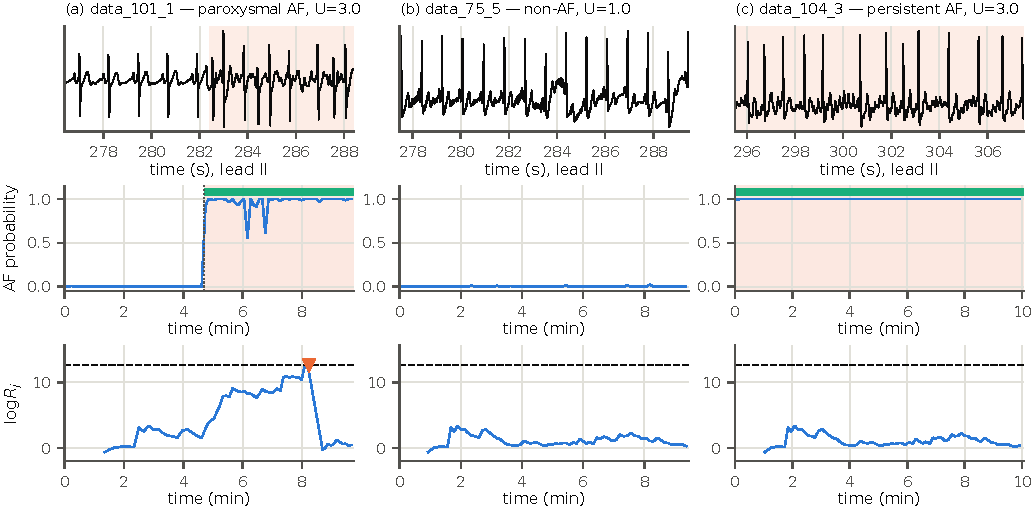
\includegraphics[width=\textwidth]{figures/fig_traces.pdf}
\caption{Example recordings (fold-1 test patients, seed 0). The top row shows lead~II at the first transition, the middle row the block AF probability, reference AF (shaded), episodes (bar) and boundaries (dotted), and the bottom row $\log R_j$, $\log A$ (dashed) and the alarm (triangle).}
\label{fig:traces}
\end{figure*}

\begin{figure*}[!htbp]
\centering
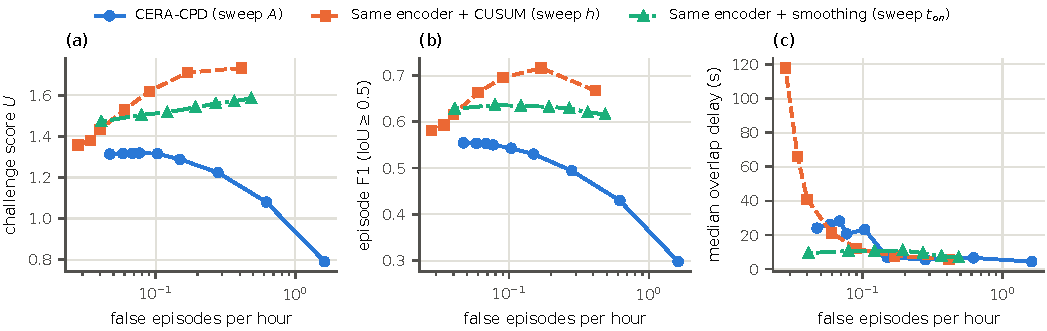
\includegraphics[width=\textwidth]{figures/fig_operating.pdf}
\caption{Operating curves on the CPSC2021 test folds (mean of five seeds), one point per threshold ($A$, the CUSUM threshold $h$ or the smoothing threshold $t_{\mathrm{on}}$), showing (a) challenge score, (b) episode F1 and (c) median overlap-based delay versus false episodes per hour.}
\label{fig:operating}
\end{figure*}

In zero-shot transfer (Table~\ref{tab:external}), CUSUM (AFDB episode F1 57.4\%) and smoothing (55.3\%) again outperformed \method{} (15.6\%), whose false-episode rate was the lowest (0.02 per hour) but whose burden error was larger (15.9 percentage points) because long episodes were detected late. LTAFDB was difficult for every method, because 35\% of its 7358 episodes are shorter than one block. The best episode F1 was 11.8\% (CUSUM), although burden errors stayed small for CUSUM and smoothing (3.7 and 2.7 percentage points). In EC57 terms (Table~\ref{tab:ec57}), CUSUM detected 96.8\% of CPSC2021 AF time at an AF-time specificity of 98.6\% and overlapped 95.6\% of the episodes lasting at least 30\,s, against 87.9\%, 96.6\% and 81.5\% for \method{}, while \method{}-G matched CUSUM. The 30-s criterion removed 79\% of the false episodes of the percentile rule but at most a fifth of those of the sequential detectors, whose false episodes rarely lasted less than 30\,s.

\begin{table*}[!htbp]
\centering
\caption{Zero-shot external testing. Bnd.\ Se is the boundary sensitivity within $\pm2$ beats (\%), FA/h the false episodes per hour, Burden the mean absolute error (percentage points) and Cov./width the coverage/width (\%) of 90\% intervals, bounded for incomplete labels. $^\dagger$Offline. Bold marks the best online value.}
\label{tab:external}
\footnotesize
\setlength{\tabcolsep}{3pt}
\par\smallskip
\textbf{(a) AFDB (23 recordings, 234\,h)}
\par\smallskip
\fitwidth{%
\begin{tabular}{@{}lccccc@{}}
\toprule
Method & Ep.\ F1 & Bnd.\ Se & FA/h & Burden & Cov./width\\
\midrule
COSEn & 33.1\,$\pm$\,8.8 & 23.9\,$\pm$\,7.3 & 0.63\,$\pm$\,0.42 & 3.8\,$\pm$\,1.6 & 96/52\\
RR Markov & 26.5\,$\pm$\,8.7 & 13.1\,$\pm$\,5.7 & 1.01\,$\pm$\,0.69 & 7.4\,$\pm$\,2.6 & 96/73\\
RR-LSTM & 39.9\,$\pm$\,20.2 & 2.1\,$\pm$\,1.5 & 0.09\,$\pm$\,0.05 & 9.0\,$\pm$\,11.5 & 96/62\\
1-D U-Net$^\dagger$ & 44.1\,$\pm$\,9.3 & 22.5\,$\pm$\,9.5 & 0.17\,$\pm$\,0.11 & 3.9\,$\pm$\,2.0 & 97/71\\
Causal smoothing & 55.3\,$\pm$\,9.7 & 35.0\,$\pm$\,9.3 & 0.12\,$\pm$\,0.20 & \textbf{2.5\,$\pm$\,0.9} & 99/48\\
CUSUM & \textbf{57.4\,$\pm$\,12.7} & \textbf{37.0\,$\pm$\,8.4} & 0.06\,$\pm$\,0.09 & 5.3\,$\pm$\,2.7 & 94/44\\
BOCPD & 43.5\,$\pm$\,5.9 & 26.3\,$\pm$\,6.6 & 0.06\,$\pm$\,0.04 & 17.5\,$\pm$\,3.5 & 89/72\\
\method{}, $\lambda^\star=0.1$/h & 16.3\,$\pm$\,1.5 & 5.3\,$\pm$\,0.7 & \textbf{0.02\,$\pm$\,0.01} & 17.9\,$\pm$\,3.4 & 95/91\\
\method{}, validated $A$ & 15.6\,$\pm$\,1.6 & 5.0\,$\pm$\,1.4 & \textbf{0.02\,$\pm$\,0.03} & 15.9\,$\pm$\,3.8 & 97/95\\
\bottomrule
\end{tabular}}
\par\smallskip
\textbf{(b) LTAFDB (84 recordings, 1961\,h)}
\par\smallskip
\fitwidth{%
\begin{tabular}{@{}lccccc@{}}
\toprule
Method & Ep.\ F1 & Bnd.\ Se & FA/h & Burden & Cov./width\\
\midrule
COSEn & 9.2\,$\pm$\,0.6 & 3.3\,$\pm$\,0.4 & 0.81\,$\pm$\,0.42 & 3.3\,$\pm$\,0.8 & [93.1, 94.0]/46\\
RR Markov & 6.9\,$\pm$\,1.7 & 2.1\,$\pm$\,0.6 & 0.62\,$\pm$\,0.22 & 7.5\,$\pm$\,3.5 & [93.6, 94.0]/71\\
RR-LSTM & 7.3\,$\pm$\,3.4 & 0.6\,$\pm$\,0.4 & 0.09\,$\pm$\,0.06 & 7.5\,$\pm$\,6.8 & [94.5, 95.2]/57\\
1-D U-Net$^\dagger$ & 10.0\,$\pm$\,2.5 & 3.1\,$\pm$\,1.7 & 0.14\,$\pm$\,0.07 & 5.7\,$\pm$\,2.0 & [96.7, 97.3]/66\\
Causal smoothing & 10.9\,$\pm$\,3.4 & \textbf{4.6\,$\pm$\,2.7} & 0.07\,$\pm$\,0.11 & \textbf{2.7\,$\pm$\,1.4} & [96.6, 97.7]/40\\
CUSUM & \textbf{11.8\,$\pm$\,3.7} & 4.4\,$\pm$\,2.0 & \textbf{0.02\,$\pm$\,0.02} & 3.7\,$\pm$\,1.7 & [94.5, 95.5]/36\\
BOCPD & 5.9\,$\pm$\,2.5 & 2.5\,$\pm$\,1.1 & \textbf{0.02\,$\pm$\,0.01} & 13.4\,$\pm$\,2.9 & [90.4, 91.4]/63\\
\method{}, $\lambda^\star=0.1$/h & 2.7\,$\pm$\,0.2 & 0.8\,$\pm$\,0.1 & \textbf{0.02\,$\pm$\,0.01} & 16.1\,$\pm$\,2.5 & [96.8, 96.9]/88\\
\method{}, validated $A$ & 2.4\,$\pm$\,0.5 & 0.7\,$\pm$\,0.3 & \textbf{0.02\,$\pm$\,0.03} & 15.9\,$\pm$\,3.7 & [98.7, 98.8]/93\\
\bottomrule
\end{tabular}}
\end{table*}


\begin{table*}[!htbp]
\centering
\caption{EC57-style metrics (\%), namely AF-time Se/PPV/Sp on labelled time, any-overlap episode Se/PPV, Se for episodes of at least 30\,s and their false episodes per hour (FA$_{30}$/h), with burden agreement given as Bland and Altman bias [95\% limits] (percentage points) and Lin's CCC. $^\dagger$Offline. Bold marks the best online value.}
\label{tab:ec57}
\footnotesize
\setlength{\tabcolsep}{3pt}
\par\smallskip
\textbf{(a) CPSC2021 cross-validation}
\par\smallskip
\fitwidth{%
\begin{tabular}{@{}>{\raggedright\arraybackslash}p{4.3cm}ccccccc@{}}
\toprule
Method & AF-time Se & AF-time PPV & AF-time Sp & Ep.\ Se & Ep.\ PPV & Se$_{\ge30\,\mathrm{s}}$ & FA$_{30}$/h\\
\midrule
\multicolumn{8}{@{}l}{\textit{Rhythm features}}\\
CV of RR \cite{tateno2001} & 77.8 & 63.2 & 76.3 & 86.7 & 57.1 & 89.1 & 2.068\\
COSEn \cite{lake2011cosen} & \textbf{97.8} & 90.2 & 94.4 & 69.3 & 49.6 & 98.2 & 1.041\\
RR Markov \cite{moody1983afdb} & 94.9 & 78.7 & 86.6 & 70.3 & 53.7 & 95.4 & 1.562\\
\midrule
\multicolumn{8}{@{}l}{\textit{Deep sequence}}\\
RR-LSTM, causal \cite{faust2018} & 95.6\,$\pm$\,0.3 & 92.5\,$\pm$\,0.7 & 95.9\,$\pm$\,0.4 & 63.3\,$\pm$\,4.6 & 69.6\,$\pm$\,2.9 & 89.8\,$\pm$\,1.2 & 0.450\,$\pm$\,0.043\\
1-D U-Net, offline$^\dagger$ \cite{wen2022paf} & 95.0\,$\pm$\,1.0 & 87.9\,$\pm$\,3.7 & 93.1\,$\pm$\,2.4 & 59.0\,$\pm$\,2.1 & 66.4\,$\pm$\,0.9 & 91.6\,$\pm$\,1.9 & 0.616\,$\pm$\,0.027\\
\midrule
\multicolumn{8}{@{}l}{\textit{Same encoder}}\\
Causal smoothing & 97.5\,$\pm$\,0.3 & 96.2\,$\pm$\,0.5 & 98.0\,$\pm$\,0.3 & 73.1\,$\pm$\,2.6 & 88.3\,$\pm$\,1.7 & 97.2\,$\pm$\,0.4 & 0.127\,$\pm$\,0.022\\
Percentile threshold & 96.8\,$\pm$\,0.2 & 95.4\,$\pm$\,0.1 & 97.6\,$\pm$\,0.1 & \textbf{88.9\,$\pm$\,0.6} & 64.8\,$\pm$\,0.9 & \textbf{99.1\,$\pm$\,0.1} & 0.355\,$\pm$\,0.023\\
CUSUM \cite{page1954} & 96.8\,$\pm$\,0.5 & \textbf{97.4\,$\pm$\,0.2} & \textbf{98.6\,$\pm$\,0.1} & 72.0\,$\pm$\,2.1 & 95.0\,$\pm$\,1.1 & 95.6\,$\pm$\,0.5 & 0.068\,$\pm$\,0.005\\
BOCPD \cite{adams2007bocpd} & 87.9\,$\pm$\,1.0 & 93.3\,$\pm$\,0.7 & 96.7\,$\pm$\,0.4 & 67.9\,$\pm$\,1.8 & \textbf{95.8\,$\pm$\,0.9} & 89.8\,$\pm$\,0.7 & \textbf{0.060\,$\pm$\,0.014}\\
\midrule
\multicolumn{8}{@{}l}{\textit{Proposed}}\\
\method{}, validated $A$ & 87.9\,$\pm$\,1.5 & 93.1\,$\pm$\,1.3 & 96.6\,$\pm$\,0.7 & 59.6\,$\pm$\,2.1 & 94.2\,$\pm$\,1.4 & 81.5\,$\pm$\,1.0 & 0.069\,$\pm$\,0.018\\
\method{}-G, validated & 96.8\,$\pm$\,0.5 & 97.3\,$\pm$\,0.2 & \textbf{98.6\,$\pm$\,0.1} & 67.0\,$\pm$\,2.2 & 95.4\,$\pm$\,0.6 & 94.6\,$\pm$\,0.7 & 0.066\,$\pm$\,0.008\\
\bottomrule
\end{tabular}}
\par\smallskip
\textbf{(b) Burden agreement}
\par\smallskip
\fitwidth{%
\begin{tabular}{@{}>{\raggedright\arraybackslash}p{4.3cm}cccc@{}}
\toprule
 & \multicolumn{2}{c}{CPSC2021 (pre-selected recordings)} & \multicolumn{2}{c}{AFDB}\\
\cmidrule(lr){2-3}\cmidrule(lr){4-5}
Method & Bias [95\% LoA] & CCC & Bias [95\% LoA] & CCC\\
\midrule
CV of RR \cite{tateno2001} & +7.9 [$-$75.9, 91.6] & 0.51 & $-$6.8 [$-$53.7, 40.1] & 0.69\\
COSEn \cite{lake2011cosen} & +1.9 [$-$28.4, 32.3] & 0.94 & $-$2.2 [$-$20.1, 15.6] & 0.96\\
RR Markov \cite{moody1983afdb} & +6.2 [$-$41.8, 54.2] & 0.84 & $-$2.2 [$-$30.1, 25.7] & 0.89\\
RR-LSTM, causal \cite{faust2018} & +0.4 [$-$29.9, 30.7] & 0.94 & $-$8.5 [$-$32.2, 15.2] & 0.85\\
1-D U-Net, offline$^\dagger$ \cite{wen2022paf} & +1.4 [$-$34.9, 37.8] & 0.92 & $-$3.1 [$-$17.6, 11.4] & 0.97\\
Causal smoothing & +1.2 [$-$30.9, 33.3] & 0.94 & \textbf{$-$1.7 [$-$12.6, 9.1]} & \textbf{0.98}\\
Percentile threshold & +0.6 [$-$28.9, 30.0] & \textbf{0.95} & $-$2.3 [$-$13.9, 9.4] & \textbf{0.98}\\
CUSUM \cite{page1954} & \textbf{+0.2 [$-$29.9, 30.2]} & 0.94 & $-$5.1 [$-$30.8, 20.6] & 0.90\\
BOCPD \cite{adams2007bocpd} & $-$1.3 [$-$46.1, 43.5] & 0.87 & $-$12.5 [$-$66.6, 41.6] & 0.56\\
\method{}, validated $A$ & $-$3.5 [$-$52.0, 45.0] & 0.85 & $-$7.9 [$-$57.8, 42.1] & 0.64\\
\method{}-G, validated & +0.4 [$-$29.4, 30.1] & \textbf{0.95} & $-$5.8 [$-$38.8, 27.2] & 0.85\\
\bottomrule
\end{tabular}}
\end{table*}

\begin{table*}[!htbp]
\ContinuedFloat
\centering
\caption[]{Standard AF-detector metrics (continued) for zero-shot external testing.}
\footnotesize
\setlength{\tabcolsep}{3pt}
\par\smallskip
\textbf{(c) AFDB, zero-shot (23 recordings)}
\par\smallskip
\fitwidth{%
\begin{tabular}{@{}>{\raggedright\arraybackslash}p{4.3cm}ccccccc@{}}
\toprule
Method & AF-time Se & AF-time PPV & AF-time Sp & Ep.\ Se & Ep.\ PPV & Se$_{\ge30\,\mathrm{s}}$ & FA$_{30}$/h\\
\midrule
\multicolumn{8}{@{}l}{\textit{Rhythm features}}\\
CV of RR \cite{tateno2001} & 70.6 & 85.0 & 91.4 & 90.2 & 67.2 & 92.9 & 1.187\\
COSEn \cite{lake2011cosen} & 91.9 & 97.4 & 98.3 & 83.5 & 79.8 & 97.1 & 0.254\\
RR Markov \cite{moody1983afdb} & 87.3 & 92.9 & 95.0 & 84.7 & 72.2 & 95.0 & 0.739\\
\midrule
\multicolumn{8}{@{}l}{\textit{Deep sequence}}\\
RR-LSTM, causal \cite{faust2018} & 77.6 & 98.3 & 99.1 & 61.0 & 89.7 & 72.9 & 0.063\\
1-D U-Net, offline$^\dagger$ \cite{wen2022paf} & 90.6 & 98.1 & 98.8 & 75.8 & 89.5 & 88.9 & 0.104\\
\midrule
\multicolumn{8}{@{}l}{\textit{Same encoder}}\\
Causal smoothing & \textbf{94.3} & 98.5 & 99.0 & 79.9 & 93.6 & 94.2 & 0.041\\
Percentile threshold & 92.6 & 98.1 & 98.8 & \textbf{91.7} & 78.8 & \textbf{97.8} & 0.149\\
CUSUM \cite{page1954} & 86.8 & \textbf{99.3} & \textbf{99.6} & 72.2 & 97.0 & 86.5 & 0.020\\
BOCPD \cite{adams2007bocpd} & 58.4 & 84.7 & 92.8 & 63.0 & 93.3 & 69.7 & 0.056\\
\midrule
\multicolumn{8}{@{}l}{\textit{Proposed}}\\
\method{}, validated $A$ & 67.7 & 84.2 & 91.3 & 50.3 & 94.7 & 56.0 & \textbf{0.018}\\
\method{}-G, validated & 84.9 & 99.2 & 99.5 & 70.0 & \textbf{97.9} & 84.5 & \textbf{0.018}\\
\bottomrule
\end{tabular}}
\par\smallskip
\textbf{(d) LTAFDB, zero-shot (84 recordings)}
\par\smallskip
\fitwidth{%
\begin{tabular}{@{}>{\raggedright\arraybackslash}p{4.3cm}ccccccc@{}}
\toprule
Method & AF-time Se & AF-time PPV & AF-time Sp & Ep.\ Se & Ep.\ PPV & Se$_{\ge30\,\mathrm{s}}$ & FA$_{30}$/h\\
\midrule
\multicolumn{8}{@{}l}{\textit{Rhythm features}}\\
CV of RR \cite{tateno2001} & 68.3 & 82.6 & 84.1 & \textbf{87.5} & 82.3 & 90.8 & 0.732\\
COSEn \cite{lake2011cosen} & 96.2 & 96.2 & 95.6 & 69.0 & 62.9 & 95.7 & 0.377\\
RR Markov \cite{moody1983afdb} & 91.2 & 93.1 & 91.8 & 79.0 & 73.0 & \textbf{96.4} & 0.500\\
\midrule
\multicolumn{8}{@{}l}{\textit{Deep sequence}}\\
RR-LSTM, causal \cite{faust2018} & 86.7 & 98.6 & 98.6 & 47.8 & 87.6 & 74.2 & 0.070\\
1-D U-Net, offline$^\dagger$ \cite{wen2022paf} & 90.5 & 97.8 & 97.7 & 55.8 & 88.2 & 85.1 & 0.113\\
\midrule
\multicolumn{8}{@{}l}{\textit{Same encoder}}\\
Causal smoothing & \textbf{96.3} & 98.2 & 97.9 & 62.8 & 93.1 & 91.5 & 0.039\\
Percentile threshold & 95.8 & 98.0 & 97.8 & 71.2 & 83.1 & 96.0 & 0.165\\
CUSUM \cite{page1954} & 94.0 & \textbf{98.8} & \textbf{98.7} & 54.7 & 97.5 & 84.4 & 0.013\\
BOCPD \cite{adams2007bocpd} & 77.3 & 93.4 & 93.6 & 50.2 & 94.5 & 67.0 & 0.017\\
\midrule
\multicolumn{8}{@{}l}{\textit{Proposed}}\\
\method{}, validated $A$ & 79.1 & 87.6 & 87.1 & 55.2 & 89.2 & 64.6 & 0.020\\
\method{}-G, validated & 94.0 & \textbf{98.8} & \textbf{98.7} & 54.0 & \textbf{97.9} & 83.6 & \textbf{0.009}\\
\bottomrule
\end{tabular}}
\end{table*}


\subsection{False-Alarm Control and Robustness}
\label{sec:res-fa}
\label{sec:res-robust}
Fig.~\ref{fig:fa}(a) is consistent with the fixed-mode guarantee (H2). For exchangeable scores, the restricted mean run length exceeded $A$ by a factor of 3.8 to 6.3 for $A=10$ to $10^3$, and repeated alarms with resets stayed far below the bound \eqref{eq:alarmcount} (3.0 vs 19.9 alarms in $2\times10^4$ blocks at $A=10^3$). With AR(1) scores, the ratio fell to 0.51 ($\rho=0.5$) and 0.11 ($\rho=0.9$), and repeated alarms exceeded the bound (35.4 and 86.6). Real ECG lies between these regimes. Raw fused logits on NSRDB were strongly autocorrelated (median lag-1 autocorrelation 0.62), but after decision clipping almost all null scores were tied at zero and their autocorrelation was 0.02. The nominal budgets of 1 and 0.1 alarms per hour were met on NSRDB (median 0.22 and 0.085, Fig.~\ref{fig:fa}b), with similar rates on other non-AF recordings, whereas for $A\ge3\times10^4$ the rate levelled off near 0.05 per hour. In false episodes per hour (Table~\ref{tab:controls}), \method{} (0.05 on NSRDB and 0.16 to 0.18 on MIT-BIH non-AF) was comparable to CUSUM and BOCPD, three to four times lower than smoothing on ectopy-rich recordings and 5- to 55-fold lower than the RR detectors and the U-Net.

\begin{figure*}[!htbp]
\centering
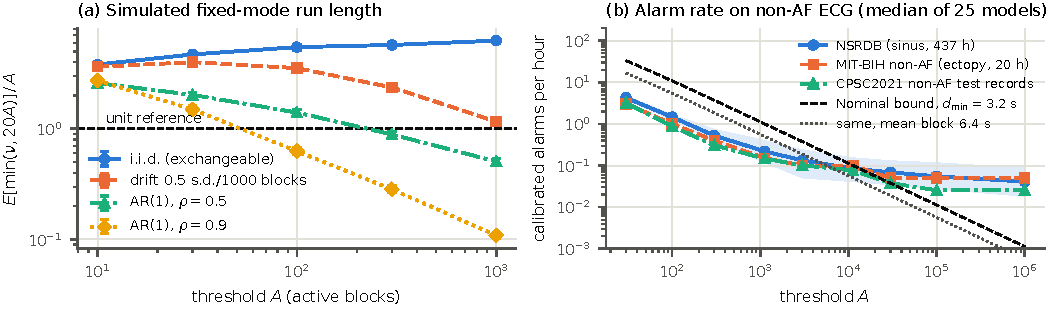
\includegraphics[width=\textwidth]{figures/fig_false_alarms.pdf}
\caption{False-alarm control, showing (a) restricted mean run length divided by $A$ (95\% intervals) for exchangeable, drifting and AR(1) scores and (b) calibrated alarms per hour versus $A$ on non-AF recordings (median, with the NSRDB range as band) with nominal bounds.}
\label{fig:fa}
\end{figure*}

\begin{table}[!htbp]
\centering
\caption{False episodes per hour on change-free and ectopy-rich recordings (mean\,$\pm$\,s.d.\ over locked models). Bold marks the best value.}
\label{tab:controls}
\footnotesize
\setlength{\tabcolsep}{3pt}
\begin{tabular}{@{}lcc@{}}
\toprule
Method & NSRDB (437\,h) & MIT-BIH non-AF (20\,h)\\
\midrule
COSEn & 2.75\,$\pm$\,1.31 & 4.96\,$\pm$\,1.61\\
RR Markov & 0.70\,$\pm$\,0.49 & 1.98\,$\pm$\,1.49\\
RR-LSTM & 0.07\,$\pm$\,0.06 & 0.59\,$\pm$\,0.45\\
1-D U-Net$^\dagger$ & 0.42\,$\pm$\,0.88 & 0.85\,$\pm$\,0.59\\
Causal smoothing & 0.06\,$\pm$\,0.08 & 0.65\,$\pm$\,0.65\\
CUSUM & \textbf{0.03\,$\pm$\,0.03} & 0.20\,$\pm$\,0.15\\
BOCPD & \textbf{0.03\,$\pm$\,0.03} & 0.23\,$\pm$\,0.16\\
\method{}, $\lambda^\star=0.1$/h & 0.05\,$\pm$\,0.02 & \textbf{0.16\,$\pm$\,0.13}\\
\method{}, validated $A$ & 0.05\,$\pm$\,0.07 & 0.18\,$\pm$\,0.17\\
\method{} w/o ectopy sampling & n/a & 0.17\,$\pm$\,0.10\\
\bottomrule
\end{tabular}
\end{table}


Noise stress exposed the main strength of patient-adaptive calibration (Fig.~\ref{fig:noise}, Table~\ref{tab:s-noise}). Electrode motion at 0\,dB reduced the episode F1 of CUSUM from 73.0\% to 44.1\% and raised its false episodes from 0.09 to 0.31 per hour (smoothing 0.93), whereas \method{} remained stable (F1 45.9\% clean and 51.8\% at 0\,dB, with 0.04 to 0.08 false episodes per hour). Muscle artefact lowered F1 without raising false alarms, and baseline wander had little effect. The noise component of H2 was only weakly supported, since the learned gate produced fewer false episodes than equal weights in clean data (0.042 vs 0.057 per hour) and in six of nine noisy conditions, but by at most 0.02 per hour. The ectopy component was not supported robustly. Removing ectopy-nuisance sampling increased false episodes on ectopy-rich CPSC2021 recordings from 0.10 to 0.15 per hour but not on MIT-BIH, whereas removing the atrial stream tripled them (Table~\ref{tab:ablation}).

\begin{figure*}[!htbp]
\centering
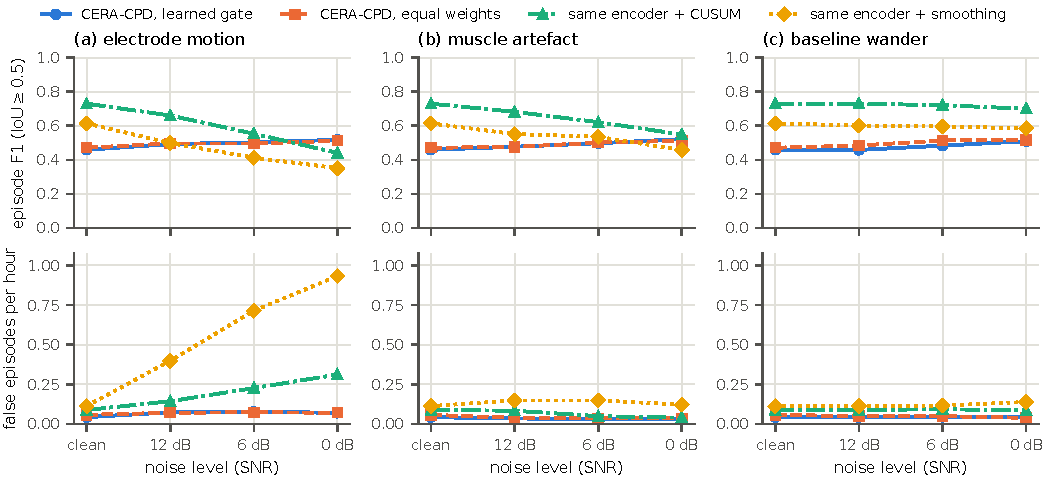
\includegraphics[width=\textwidth]{figures/fig_noise.pdf}
\caption{NSTDB noise stress on the 105 pre-selected CPSC2021 recordings, each scored by the models of its own test fold (mean of five seeds, three for equal weights), with episode F1 at the top and false episodes per hour at the bottom.}
\label{fig:noise}
\end{figure*}

\begin{table*}[!htbp]
\centering
\caption{Noise stress on the 105 pre-selected CPSC2021 recordings, given as episode F1 (\%) / false episodes per hour (mean over seeds, each recording scored only by its own fold's models). Bold marks the best F1 and FA/h.}
\label{tab:s-noise}
\footnotesize
\setlength{\tabcolsep}{2.5pt}
\par\smallskip
\textbf{(a) Clean ECG}
\par\smallskip
\fitwidth{%
\begin{tabular}{@{}p{5cm}c@{}}
\toprule
Method & Clean\\
\midrule
\method{} & 45.9/\textbf{0.04}\\
\method{}, equal weights & 47.1/0.06\\
CUSUM & \textbf{73.0}/0.09\\
Smoothing & 61.4/0.11\\
\bottomrule
\end{tabular}}
\par\smallskip
\textbf{(b) Electrode motion (em)}
\par\smallskip
\fitwidth{%
\begin{tabular}{@{}p{5cm}ccc@{}}
\toprule
Method & 12\,dB & 6\,dB & 0\,dB\\
\midrule
\method{} & 49.3/\textbf{0.07} & 50.3/0.08 & \textbf{51.8}/\textbf{0.07}\\
\method{}, equal weights & 49.6/\textbf{0.07} & 49.6/\textbf{0.07} & 51.3/\textbf{0.07}\\
CUSUM & \textbf{66.1}/0.14 & \textbf{55.3}/0.23 & 44.1/0.31\\
Smoothing & 49.8/0.40 & 41.3/0.71 & 35.1/0.93\\
\bottomrule
\end{tabular}}
\par\smallskip
\textbf{(c) Muscle artefact (ma)}
\par\smallskip
\fitwidth{%
\begin{tabular}{@{}p{5cm}ccc@{}}
\toprule
Method & 12\,dB & 6\,dB & 0\,dB\\
\midrule
\method{} & 47.7/\textbf{0.03} & 49.8/\textbf{0.03} & 52.2/\textbf{0.03}\\
\method{}, equal weights & 47.6/0.04 & 50.1/0.04 & 51.2/0.04\\
CUSUM & \textbf{68.2}/0.08 & \textbf{62.2}/0.05 & \textbf{54.9}/0.04\\
Smoothing & 55.1/0.15 & 53.5/0.15 & 45.8/0.12\\
\bottomrule
\end{tabular}}
\par\smallskip
\textbf{(d) Baseline wander (bw)}
\par\smallskip
\fitwidth{%
\begin{tabular}{@{}p{5cm}ccc@{}}
\toprule
Method & 12\,dB & 6\,dB & 0\,dB\\
\midrule
\method{} & 45.8/\textbf{0.04} & 48.3/\textbf{0.04} & 51.0/\textbf{0.04}\\
\method{}, equal weights & 48.4/0.05 & 51.4/0.05 & 51.6/\textbf{0.04}\\
CUSUM & \textbf{73.0}/0.09 & \textbf{72.1}/0.09 & \textbf{70.0}/0.08\\
Smoothing & 60.1/0.11 & 59.5/0.12 & 58.6/0.14\\
\bottomrule
\end{tabular}}
\end{table*}


With causal QRS detection (Table~\ref{tab:qrs}), sensitivity was 97.6 to 99.9\% and positive predictivity 95.9 to 99.3\% on clean recordings (median confirmation latency 0.24\,s). At 0\,dB electrode motion and muscle noise, 25 to 31\% of the detections were spurious. Automatic detection lowered the challenge score of every detector by 0.04 to 0.19, mainly through beat-level boundary credit, but CUSUM, causal smoothing and \method{}-G kept the three highest scores. CUSUM remained ahead of \method{} ($U=1.51$ vs 1.22, $\Delta U=-0.22$, $[-0.34,-0.11]$), and gating it reduced false episodes from 0.115 to 0.075 per hour ($p<0.001$) at a cost of 0.04 in the score. Noise widened the differences on this track because detection errors also corrupt the RR features (Fig.~\ref{fig:noise-qrs}). At 0\,dB electrode motion, false episodes rose to 0.46 per hour for CUSUM, 2.25 for smoothing and 5.97 for COSEn, whereas \method{} remained at 0.09 with an episode F1 of 46.5\%, against 28.8\% for CUSUM (difference $-0.59$ false episodes per hour, $p<0.001$), and the certificate $A_c=1121$ gave the highest challenge score (0.99 vs 0.88).

\begin{table*}[!htbp]
\centering
\caption{End-to-end track with causal QRS detection, showing (a) detection accuracy and latency ($^\ddagger$largely automatic reference beats) and (b) delineation with locked settings, with CPSC2021 reference-peak values in parentheses. F1 is in \% and FA/h denotes false episodes per hour. Bold marks the best value in (b).}
\label{tab:qrs}
\footnotesize
\setlength{\tabcolsep}{3pt}
\par\smallskip
\textbf{(a) QRS detection}
\par\smallskip
\fitwidth{%
\begin{tabular}{@{}lrrccc@{}}
\toprule
Recordings & Records & Reference beats & Se (\%) & PPV (\%) & Latency (s)\\
\midrule
CPSC2021 & 1425 & 2\,122\,819 & 99.48 & 97.94 & 0.24\\
AFDB$^\ddagger$ & 23 & 1\,130\,172 & 97.58 & 97.25 & 0.24\\
LTAFDB & 84 & 8\,995\,973 & 99.69 & 95.85 & 0.24\\
NSRDB & 18 & 1\,729\,629 & 99.91 & 99.30 & 0.24\\
MIT-BIH Arrhythmia & 48 & 109\,494 & 99.85 & 99.14 & 0.23\\
CPSC2021 pre-selected (clean) & 105 & 556\,146 & 99.43 & 97.92 & 0.24\\
\quad electrode motion 12\,dB & 105 & 556\,146 & 99.43 & 97.07 & 0.24\\
\quad electrode motion 6\,dB & 105 & 556\,146 & 99.42 & 88.76 & 0.24\\
\quad electrode motion 0\,dB & 105 & 556\,146 & 98.10 & 69.34 & 0.24\\
\quad muscle artefact 0\,dB & 105 & 556\,146 & 98.31 & 75.10 & 0.24\\
\quad baseline wander 0\,dB & 105 & 556\,146 & 99.43 & 97.69 & 0.24\\
\bottomrule
\end{tabular}}
\par\smallskip
\textbf{(b) Delineation on detected beats}
\par\smallskip
\fitwidth{%
\begin{tabular}{@{}>{\raggedright\arraybackslash}p{4.3cm}ccccccc@{}}
\toprule
 & \multicolumn{3}{c}{CPSC2021 (CV)} & AFDB & NSRDB & \multicolumn{2}{c}{Electrode motion 0\,dB}\\
\cmidrule(lr){2-4}\cmidrule(lr){5-5}\cmidrule(lr){6-6}\cmidrule(lr){7-8}
Method & $U$ & Ep.\ F1 & FA/h & Ep.\ F1 & FA/h & Ep.\ F1 & FA/h\\
\midrule
COSEn & 1.25 (1.31) & 39.0 (39.7) & 2.276 (2.010) & 33.7 & 2.822 & 9.2 & 5.97\\
Causal smoothing & 1.46 (1.58) & 60.1 (65.0) & 0.267 (0.200) & 53.6 & 0.038 & 15.3 & 2.25\\
Percentile threshold & 1.39 (1.58) & 38.5 (48.8) & 1.868 (1.693) & 20.5 & 0.326 & 1.0 & 13.34\\
CUSUM & \textbf{1.51 (1.65)} & \textbf{66.7 (70.4)} & 0.115 (0.085) & 55.6 & 0.008 & 28.8 & 0.46\\
BOCPD & 1.35 (1.48) & 55.2 (58.8) & 0.086 (0.061) & 43.1 & 0.018 & 39.9 & 0.16\\
\method{}, validated $A$ & 1.22 (1.31) & 53.1 (54.8) & \textbf{0.065 (0.069)} & 15.9 & 0.043 & \textbf{46.5} & \textbf{0.09}\\
\method{}-G, validated & 1.45 (1.57) & 63.6 (66.3) & 0.075 (0.069) & \textbf{58.3} & \textbf{0.006} & 33.6 & 0.40\\
\bottomrule
\end{tabular}}
\end{table*}


\begin{figure*}[!htbp]
\centering
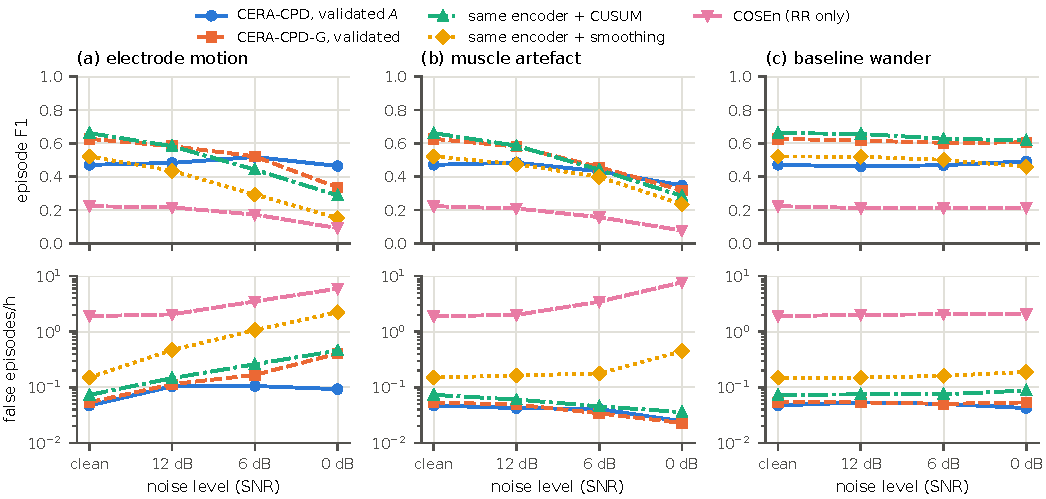
\includegraphics[width=\textwidth]{figures/fig_noise_qrs.pdf}
\caption{NSTDB noise stress on the end-to-end track, with R peaks detected from the noisy recordings (105 pre-selected CPSC2021 recordings, mean of five seeds), with episode F1 at the top and false episodes per hour (logarithmic scale) at the bottom.}
\label{fig:noise-qrs}
\end{figure*}

\subsection{AF Burden}
\label{sec:res-burden}
All 90\% split-conformal intervals attained nominal coverage on the pre-selected test recordings (93.1 to 96.8\%, Table~\ref{tab:burden}), supporting H3 for coverage, as did those recalibrated on the end-to-end track (94.2 to 96.7\%). Their usefulness depended on the detector (Fig.~\ref{fig:burden}). CUSUM gave a mean absolute error of 3.3 percentage points and a mean width of 33.0, whereas the heavy-tailed residuals of \method{} produced nearly vacuous intervals (width 82 to 87). Scaling residuals by the localisation spread reduced widths by 22 to 31\% at similar coverage. Applied unchanged, the CUSUM intervals covered 94.4\% of AFDB recordings, and LTAFDB coverage was bounded between 94.5 and 95.5\% because one recording had incomplete labels. Bland and Altman biases were small for CUSUM and \method{}-G (0.2 and 0.4 percentage points, CCC 0.94 and 0.95, Table~\ref{tab:ec57}b), with limits of about $\pm30$ points due to a few almost entirely misclassified recordings, whereas \method{} underestimated burden by 3.5 points (CCC 0.85).

\begin{table}[!htbp]
\centering
\caption{Burden on the 105 pre-selected CPSC2021 test recordings (one per patient), giving mean absolute error and coverage/mean width (percentage points) of 90\% split-conformal intervals, normalised by the localisation scale ($\omega+\epsilon$) or unnormalised. Mean over seeds. Bold marks the lowest error and width.}
\label{tab:burden}
\footnotesize
\setlength{\tabcolsep}{2.5pt}
\resizebox{\columnwidth}{!}{%
\begin{tabular}{@{}lccccc@{}}
\toprule
 & & \multicolumn{2}{c}{Normalised} & \multicolumn{2}{c}{Unnormalised}\\
\cmidrule(lr){3-4}\cmidrule(lr){5-6}
Method & MAE & Cov. (\%) & Width & Cov. (\%) & Width\\
\midrule
Causal smoothing & 3.7 & 95.8 & 35.6 & 96.4 & 51.8\\
CUSUM & \textbf{3.3} & 95.8 & \textbf{33.0} & 95.6 & \textbf{42.4}\\
BOCPD & 8.1 & 93.3 & 58.5 & 93.1 & 61.8\\
RR-LSTM & 5.1 & 94.3 & 53.0 & 94.3 & 53.0\\
\method{}, $\lambda^\star=0.1$/h & 8.8 & 96.0 & 82.1 & 95.4 & 82.1\\
\method{}, validated $A$ & 8.8 & 96.8 & 87.2 & 96.4 & 87.9\\
\bottomrule
\end{tabular}}
\end{table}


\begin{figure*}[!htbp]
\centering
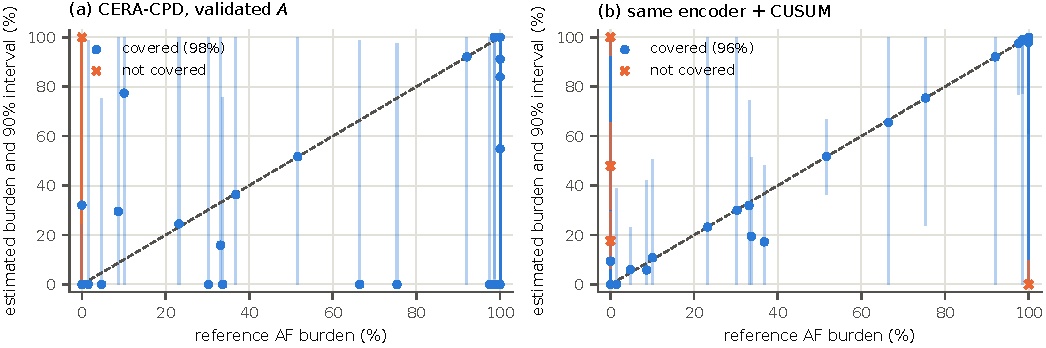
\includegraphics[width=\textwidth]{figures/fig_burden.pdf}
\caption{Estimated full-record burden and 90\% split-conformal interval versus reference burden for the 105 pre-selected CPSC2021 test recordings (seed 0) for (a) \method{} with the validated threshold and (b) the same encoder with CUSUM. The dashed line is the identity.}
\label{fig:burden}
\end{figure*}

\subsection{Detection Delay and Conformal Gating (Secondary Analyses)}
\label{sec:res-mech}
\label{sec:res-gate}
With an ideal encoder and a growing reference bag (Fig.~\ref{fig:mechanism}), the detector at a representative validated threshold ($A=3\times10^5$) never reached $\log A$ in 96 to 100\% of runs when the pre-change history held $n\le20$ blocks, in 9\% at $n=50$ and in none for $n\ge100$, whereas a fixed reference gave median post-change delays of 3 to 24 blocks. The delay is therefore caused by reference contamination and rank granularity rather than by the encoder. CPSC2021 rarely provides long histories, as 68.8\% of test onsets were preceded by fewer than 10 observed blocks and only 8.6\% by 30 or more, and within 60\,s the standalone detector alarmed for 0.0 to 3.6\% of the onsets in these strata, against 34.3 to 46.1\% for CUSUM.

\begin{figure*}[!htbp]
\centering
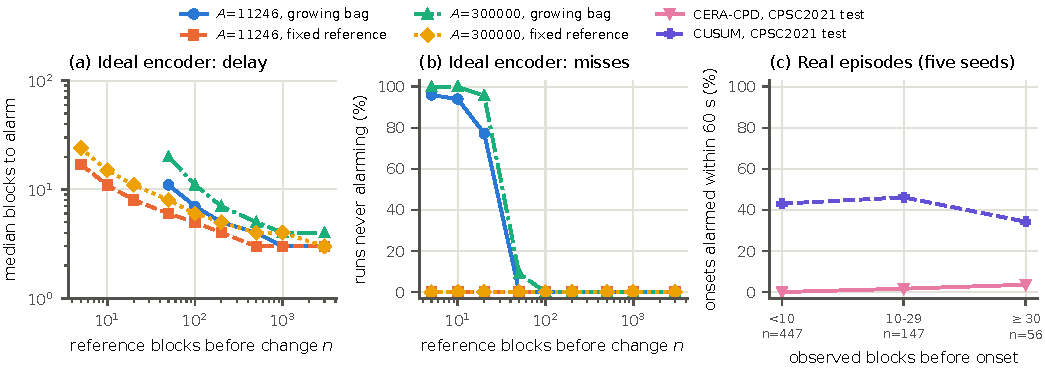
\includegraphics[width=\textwidth]{figures/fig_mechanism.pdf}
\caption{Mechanism of the detection delay, showing (a) median blocks to alarm and (b) runs without an alarm (\%) for an ideal encoder versus $n$ pre-change blocks, with growing or fixed reference, and (c) CPSC2021 onsets alarmed within 60\,s versus history blocks.}
\label{fig:mechanism}
\end{figure*}

Gating CUSUM with validated settings (Table~\ref{tab:gate}) reduced false episodes in cross-validation from 0.085 to 0.069 per hour ($\Delta=-0.024$, $[-0.049,-0.007]$, $p=0.004$) and retained most of the accuracy of CUSUM ($U=1.57$ vs 1.65, $\Delta=-0.06$, $[-0.12,-0.02]$). In zero-shot transfer it produced fewer false episodes than CUSUM on every cohort (significantly on AFDB, LTAFDB and NSRDB, $p\le0.008$), with a higher AFDB episode F1 (60.4\% vs 57.4\%) and no significant change in external burden error, and under electrode motion at 0 and 6\,dB it had the highest challenge score of all detectors (1.31 and 1.44, against 1.25 and 1.39 for CUSUM). As $A_c$ grows from 3 to $10^4$ blocks, false episodes fall from 0.077 to 0.037 per hour while the score declines from 1.59 to 1.35 (Fig.~\ref{fig:certification}). The certificate is not specific to CUSUM (Table~\ref{tab:gatex}). With the validated certificate, gating reduced the false episodes of causal smoothing from 0.200 to 0.145 per hour, of the percentile rule from 1.693 to 0.359 and of the separately trained RR-LSTM from 0.601 to 0.199 (all $p<0.001$), raising the score of the RR-LSTM from 1.18 to 1.35, and the fixed certificate $A_c=1121$ reduced false episodes for every proposer on every cohort ($p\le0.005$).

\begin{table*}[!htbp]
\centering
\caption{Secondary analysis of CUSUM proposals certified by the conformal e-detector (\method{}-G). F1 is in \% and FA/h denotes false episodes per hour. Bold marks the best value, and $^\ast$ a paired difference from CUSUM with $p<0.05$, favouring CUSUM only for the CPSC2021 score.}
\label{tab:gate}
\footnotesize
\setlength{\tabcolsep}{2.5pt}
\par\smallskip
\textbf{(a) CPSC2021 cross-validation}
\par\smallskip
\fitwidth{%
\begin{tabular}{@{}p{4.6cm}ccc@{}}
\toprule
Method & $U$ & Ep.\ F1 & FA/h\\
\midrule
Same encoder + CUSUM (best baseline) & \textbf{1.65\,$\pm$\,0.03} & \textbf{70.4\,$\pm$\,1.2} & 0.085\,$\pm$\,0.020\\
\method{} (standalone, validated $A$) & 1.31\,$\pm$\,0.02 & 54.8\,$\pm$\,0.6 & 0.069\,$\pm$\,0.018\\
\method{}-G (gated, validated) & 1.57\,$\pm$\,0.03$^\ast$ & 66.3\,$\pm$\,0.8 & 0.069\,$\pm$\,0.010$^\ast$\\
\method{}-G, certified $A_c=1121$ & 1.37\,$\pm$\,0.01 & 57.0\,$\pm$\,0.2 & \textbf{0.043\,$\pm$\,0.006}\\
\bottomrule
\end{tabular}}
\par\smallskip
\textbf{(b) External cohorts}
\par\smallskip
\fitwidth{%
\begin{tabular}{@{}p{4.6cm}ccccc@{}}
\toprule
Method & \shortstack{AFDB\\Ep.\ F1} & \shortstack{AFDB\\FA/h} & \shortstack{LTAFDB\\FA/h} & \shortstack{NSRDB\\FA/h} & \shortstack{MIT-BIH non-AF\\FA/h}\\
\midrule
Same encoder + CUSUM (best baseline) & 57.4 & 0.060 & 0.018 & 0.028 & 0.20\\
\method{} (standalone, validated $A$) & 15.6 & 0.018 & 0.020 & 0.055 & 0.18\\
\method{}-G (gated, validated) & \textbf{60.4} & 0.031$^\ast$ & 0.011$^\ast$ & 0.018$^\ast$ & 0.17\\
\method{}-G, certified $A_c=1121$ & 24.7 & \textbf{0.006} & \textbf{0.005} & \textbf{0.011} & \textbf{0.12}\\
\bottomrule
\end{tabular}}
\par\smallskip
\textbf{(c) Electrode-motion noise at 0\,dB}
\par\smallskip
\fitwidth{%
\begin{tabular}{@{}p{7cm}cc@{}}
\toprule
Method & $U$ & FA/h\\
\midrule
Same encoder + CUSUM (best baseline) & 1.25 & 0.31\\
\method{} (standalone, validated $A$) & 1.22 & \textbf{0.07}\\
\method{}-G (gated, validated) & \textbf{1.31$^\ast$} & 0.19$^\ast$\\
\method{}-G, certified $A_c=1121$ & 1.28 & \textbf{0.07}\\
\bottomrule
\end{tabular}}
\end{table*}


\begin{figure*}[!htbp]
\centering
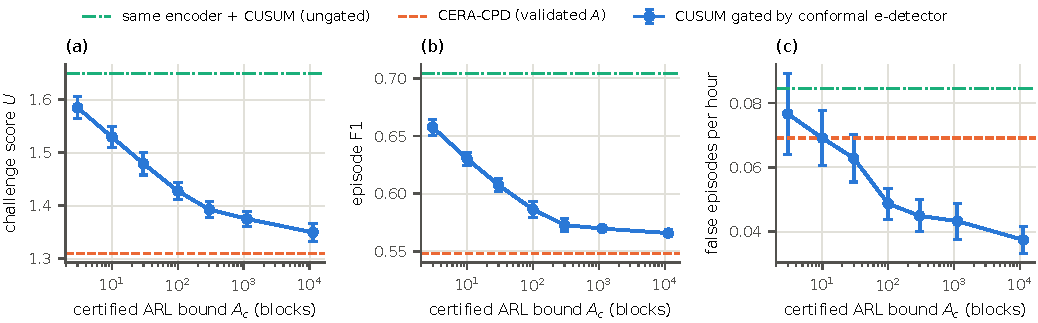
\includegraphics[width=\textwidth]{figures/fig_certification.pdf}
\caption{Price of certification on CPSC2021 (mean\,$\pm$\,s.d.\ over seeds), showing (a) challenge score, (b) episode F1 and (c) false episodes per hour of gated CUSUM proposals versus the certified ARL bound $A_c$, with ungated CUSUM and the standalone detector as references.}
\label{fig:certification}
\end{figure*}

\begin{table*}[!htbp]
\centering
\caption{Secondary analysis of the certification of further proposers with a validated or fixed ($A_c=1121$) certificate. F1 is in \% and FA/h denotes false episodes per hour, and $^\ast$ marks a paired difference from the ungated proposer with $p<0.05$. No noise scores exist for the RR-LSTM (n/a). Bold marks the best value for each proposer.}
\label{tab:gatex}
\footnotesize
\setlength{\tabcolsep}{2.5pt}
\fitwidth{%
\begin{tabular}{@{}>{\raggedright\arraybackslash}p{4.3cm}cccccccc@{}}
\toprule
 & \multicolumn{3}{c}{CPSC2021 (CV)} & AFDB & LTAFDB & NSRDB & \multicolumn{2}{c}{Electrode motion 0\,dB}\\
\cmidrule(lr){2-4}\cmidrule(lr){5-5}\cmidrule(lr){6-6}\cmidrule(lr){7-7}\cmidrule(lr){8-9}
Proposer / certificate & $U$ & Ep.\ F1 & FA/h & FA/h & FA/h & FA/h & $U$ & FA/h\\
\midrule
\multicolumn{9}{@{}l}{\textit{Causal smoothing}}\\
\quad ungated & \textbf{1.58} & \textbf{65.0} & 0.200 & 0.124 & 0.071 & 0.064 & 1.23 & 0.93\\
\quad gated, validated $A_c$ & 1.51$^\ast$ & 62.3 & 0.145$^\ast$ & 0.096$^\ast$ & 0.051$^\ast$ & 0.063 & 1.29 & 0.69\\
\quad gated, $A_c=1121$ & 1.37$^\ast$ & 56.6 & \textbf{0.057$^\ast$} & \textbf{0.011$^\ast$} & \textbf{0.010$^\ast$} & \textbf{0.023$^\ast$} & \textbf{1.33} & \textbf{0.08$^\ast$}\\
\multicolumn{9}{@{}l}{\textit{Percentile threshold}}\\
\quad ungated & \textbf{1.58} & 48.8 & 1.693 & 1.402 & 0.775 & 0.716 & 0.51 & 6.26\\
\quad gated, validated $A_c$ & 1.30 & 50.9 & 0.359$^\ast$ & 0.295$^\ast$ & 0.160$^\ast$ & 0.220$^\ast$ & 1.00$^\ast$ & 1.09$^\ast$\\
\quad gated, $A_c=1121$ & 1.33 & \textbf{54.7} & \textbf{0.103$^\ast$} & \textbf{0.039$^\ast$} & \textbf{0.027$^\ast$} & \textbf{0.073$^\ast$} & \textbf{1.21$^\ast$} & \textbf{0.14$^\ast$}\\
\multicolumn{9}{@{}l}{\textit{BOCPD}}\\
\quad ungated & \textbf{1.48} & \textbf{58.8} & 0.061 & 0.061 & 0.018 & 0.033 & 1.10 & 0.16\\
\quad gated, validated $A_c$ & 1.43$^\ast$ & 58.3 & 0.057 & 0.043$^\ast$ & 0.015$^\ast$ & 0.031 & 1.11 & 0.15\\
\quad gated, $A_c=1121$ & 1.36$^\ast$ & 56.6 & \textbf{0.033$^\ast$} & \textbf{0.013$^\ast$} & \textbf{0.005$^\ast$} & \textbf{0.011$^\ast$} & \textbf{1.24$^\ast$} & \textbf{0.06$^\ast$}\\
\multicolumn{9}{@{}l}{\textit{RR-LSTM (separate model)}}\\
\quad ungated & 1.18 & 52.8 & 0.601 & 0.087 & 0.087 & 0.066 & n/a & n/a\\
\quad gated, validated $A_c$ & \textbf{1.35$^\ast$} & \textbf{57.0} & 0.199$^\ast$ & 0.037$^\ast$ & 0.034$^\ast$ & 0.028$^\ast$ & n/a & n/a\\
\quad gated, $A_c=1121$ & 1.34$^\ast$ & 56.7 & \textbf{0.053$^\ast$} & \textbf{0.007$^\ast$} & \textbf{0.005$^\ast$} & \textbf{0.002$^\ast$} & n/a & n/a\\
\bottomrule
\end{tabular}}
\end{table*}


\subsection{Wearer Memory (Secondary Analysis)}
\label{sec:res-memory}
On CPSC2021 (Table~\ref{tab:memory}), \method{}-M raised the standalone challenge score from 1.31 to 1.44 (patient-level $\Delta=+0.085$, 95\% CI $[0.035,0.137]$, Holm-adjusted $p=0.003$) without a significant change in false episodes, and the resolution-matched calibrator raised it to 1.47 ($\Delta=+0.108$, $[0.051,0.171]$, $p<0.001$) at 0.078 false episodes per hour. Burden error fell from 7.6 to 5.5 percentage points. Validation selected margins $\gamma\ge2$ in 24 of 25 models and thresholds $A\le11246$ in 22, against $A\ge3\times10^4$ in 18 for the primary configuration. The components were complementary, since neither the margin nor memory within recordings alone changed the score significantly, and wearer memory without the margin raised false episodes to 0.108 per hour ($p<0.001$). CUSUM still scored higher ($\Delta=-0.15$, $[-0.25,-0.08]$ for \method{}-MD).

The largest change occurred on the long external recordings, where AFDB episode F1 rose from 15.6\% to 55.8\% for \method{}-M and 59.0\% for \method{}-MD, against 57.4\% for CUSUM, and \method{}-M produced fewer false episodes than CUSUM on AFDB (0.026 vs 0.060 per hour, $p=0.025$). Both variants also improved on the primary detector in LTAFDB false episodes, external burden error ($p\le0.005$) and the end-to-end score (1.34 to 1.36 vs 1.22), and stayed at 0.07 to 0.08 false episodes per hour under 0\,dB electrode motion (CUSUM 0.31), whereas on NSRDB they remained above CUSUM (Table~\ref{tab:memory}b).

The memory also lowered the price of certification (Fig.~\ref{fig:memory}). With the validated certificate ($A_c=3$ in all 25 models), \method{}-GMD matched CUSUM ($U=1.66$ vs 1.65, $p=0.74$). With $A_c=1121$, its score was 1.57 instead of 1.37 without memory ($p<0.001$), the same as that of the primary \method{}-G with $A_c=3$ at the same false-episode rate (0.068 vs 0.069 per hour). It produced fewer false episodes than CUSUM in cross-validation ($p=0.004$) and on every external cohort ($p\le0.03$), reached the highest AFDB episode F1 of all detectors (61.9\%) and under 0\,dB electrode motion matched the score of \method{}-G (1.32 vs 1.31) with 0.08 instead of 0.19 false episodes per hour, although its clean score remained below that of CUSUM ($\Delta=-0.067$, $[-0.126,-0.023]$).

\begin{table*}[!htbp]
\centering
\caption{Secondary analysis of wearer memory (validation-selected variants). F1 and boundary Se ($\pm1$ beat) are in \%, burden MAE in percentage points and FA/h denotes false episodes per hour. $^\ast$ and $^\dagger$ mark paired $p<0.05$ versus the primary configuration and CUSUM, respectively. Bold marks the best value.}
\label{tab:memory}
\footnotesize
\setlength{\tabcolsep}{2.5pt}
\par\smallskip
\textbf{(a) CPSC2021 cross-validation}
\par\smallskip
\fitwidth{%
\begin{tabular}{@{}lcccccc@{}}
\toprule
Method & $U$ & Ep.\ F1 & FA/h & Boundary Se & Burden MAE & CCC\\
\midrule
\multicolumn{7}{@{}l}{\textit{Primary configurations}}\\
\quad Same encoder + CUSUM & 1.65\,$\pm$\,0.03 & 70.4\,$\pm$\,1.2 & 0.085\,$\pm$\,0.020 & 19.0\,$\pm$\,1.9 & \textbf{3.8\,$\pm$\,0.2} & 0.94\,$\pm$\,0.00\\
\quad \method{}, validated $A$ & 1.31\,$\pm$\,0.02 & 54.8\,$\pm$\,0.6 & 0.069\,$\pm$\,0.018 & 0.8\,$\pm$\,0.2 & 7.6\,$\pm$\,0.3 & 0.85\,$\pm$\,0.02\\
\quad \method{}-G, validated $A_c$ & 1.57\,$\pm$\,0.03 & 66.3\,$\pm$\,0.8 & 0.069\,$\pm$\,0.010 & 13.0\,$\pm$\,1.7 & 4.1\,$\pm$\,0.2 & \textbf{0.95\,$\pm$\,0.00}\\
\quad \method{}-G, $A_c=1121$ & 1.37\,$\pm$\,0.01 & 57.0\,$\pm$\,0.2 & \textbf{0.043\,$\pm$\,0.006} & 2.1\,$\pm$\,0.2 & 6.8\,$\pm$\,0.2 & 0.91\,$\pm$\,0.02\\
\multicolumn{7}{@{}l}{\textit{Wearer memory}}\\
\quad \method{}-M, validated $\gamma$, $A$ & 1.44\,$\pm$\,0.02$^\ast$$^\dagger$ & 60.8\,$\pm$\,0.4 & 0.071\,$\pm$\,0.014 & 5.7\,$\pm$\,0.8 & 5.9\,$\pm$\,0.2 & 0.89\,$\pm$\,0.01\\
\quad \method{}-MD, validated $\gamma$, $A$ & 1.47\,$\pm$\,0.02$^\ast$$^\dagger$ & 61.9\,$\pm$\,0.3 & 0.078\,$\pm$\,0.006$^\ast$ & 7.4\,$\pm$\,0.7 & 5.5\,$\pm$\,0.2 & 0.90\,$\pm$\,0.02\\
\quad \method{}-GMD, validated $A_c$ & \textbf{1.66\,$\pm$\,0.02$^\ast$} & \textbf{70.9\,$\pm$\,1.1} & 0.082\,$\pm$\,0.021$^\ast$ & \textbf{19.8\,$\pm$\,1.3} & \textbf{3.8\,$\pm$\,0.2} & 0.94\,$\pm$\,0.00\\
\quad \method{}-GMD, $A_c=1121$ & 1.57\,$\pm$\,0.02$^\ast$$^\dagger$ & 66.3\,$\pm$\,0.4 & 0.068\,$\pm$\,0.010$^\ast$$^\dagger$ & 12.5\,$\pm$\,0.3 & 4.4\,$\pm$\,0.2 & 0.94\,$\pm$\,0.02\\
\multicolumn{7}{@{}l}{\textit{Ablations}}\\
\quad Margin, no memory & 1.32\,$\pm$\,0.02 & 55.4\,$\pm$\,0.5 & 0.065\,$\pm$\,0.013 & 0.9\,$\pm$\,0.1 & 7.5\,$\pm$\,0.3 & 0.86\,$\pm$\,0.02\\
\quad Margin and calibrator, no memory & 1.36\,$\pm$\,0.02$^\ast$ & 56.1\,$\pm$\,0.4 & 0.069\,$\pm$\,0.018 & 2.6\,$\pm$\,0.5 & 7.5\,$\pm$\,0.3 & 0.85\,$\pm$\,0.03\\
\quad Wearer memory, no margin & 1.39\,$\pm$\,0.03 & 57.7\,$\pm$\,1.1 & 0.108\,$\pm$\,0.011$^\ast$ & 4.9\,$\pm$\,0.7 & 6.9\,$\pm$\,0.2 & 0.87\,$\pm$\,0.02\\
\quad Memory within recordings & 1.32\,$\pm$\,0.02 & 55.8\,$\pm$\,0.5 & 0.063\,$\pm$\,0.022 & 1.1\,$\pm$\,0.4 & 7.4\,$\pm$\,0.4 & 0.86\,$\pm$\,0.02\\
\quad \method{}-G, memory within recordings & 1.58\,$\pm$\,0.03 & 67.8\,$\pm$\,0.8 & 0.074\,$\pm$\,0.011$^\ast$ & 14.3\,$\pm$\,2.1 & 4.1\,$\pm$\,0.2 & \textbf{0.95\,$\pm$\,0.00}\\
\bottomrule
\end{tabular}}
\par\smallskip
\textbf{(b) Zero-shot cohorts, noise stress and end-to-end track}
\par\smallskip
\fitwidth{%
\begin{tabular}{@{}lcccccccc@{}}
\toprule
 & \multicolumn{2}{c}{AFDB} & LTAFDB & NSRDB & MIT-BIH non-AF & \multicolumn{2}{c}{Electrode motion 0\,dB} & End-to-end\\
\cmidrule(lr){2-3}\cmidrule(lr){4-4}\cmidrule(lr){5-5}\cmidrule(lr){6-6}\cmidrule(lr){7-8}\cmidrule(lr){9-9}
Method & Ep.\ F1 & FA/h & FA/h & FA/h & FA/h & $U$ & FA/h & $U$\\
\midrule
\multicolumn{9}{@{}l}{\textit{Primary configurations}}\\
\quad Same encoder + CUSUM & 57.4 & 0.060 & 0.018 & 0.028 & 0.20 & 1.25 & 0.31 & 1.51\\
\quad \method{}, validated $A$ & 15.6 & 0.018 & 0.020 & 0.055 & 0.18 & 1.22 & \textbf{0.07} & 1.22\\
\quad \method{}-G, validated $A_c$ & 60.4 & 0.031 & 0.011 & 0.018 & 0.17 & 1.31 & 0.19 & 1.45\\
\quad \method{}-G, $A_c=1121$ & 24.7 & \textbf{0.006} & \textbf{0.005} & \textbf{0.011} & \textbf{0.12} & 1.28 & \textbf{0.07} & 1.28\\
\multicolumn{9}{@{}l}{\textit{Wearer memory}}\\
\quad \method{}-M, validated $\gamma$, $A$ & 55.8 & 0.026$^\dagger$ & 0.013$^\ast$ & 0.046 & 0.16 & 1.19 & \textbf{0.07$^\dagger$} & 1.34$^\ast$$^\dagger$\\
\quad \method{}-MD, validated $\gamma$, $A$ & 59.0 & 0.040$^\ast$ & 0.016$^\ast$ & 0.045 & 0.20 & 1.23 & 0.08$^\dagger$ & 1.36$^\ast$$^\dagger$\\
\quad \method{}-GMD, validated $A_c$ & 56.5 & 0.062$^\ast$ & 0.017$^\ast$ & 0.028$^\ast$ & 0.19 & 1.23$^\ast$ & 0.30$^\ast$ & \textbf{1.52$^\ast$}\\
\quad \method{}-GMD, $A_c=1121$ & \textbf{61.9} & 0.035$^\ast$$^\dagger$ & 0.009$^\ast$$^\dagger$ & 0.019$^\dagger$ & 0.15$^\ast$$^\dagger$ & \textbf{1.32} & 0.08$^\dagger$ & 1.45$^\ast$$^\dagger$\\
\bottomrule
\end{tabular}}
\end{table*}


\begin{figure*}[!htbp]
\centering
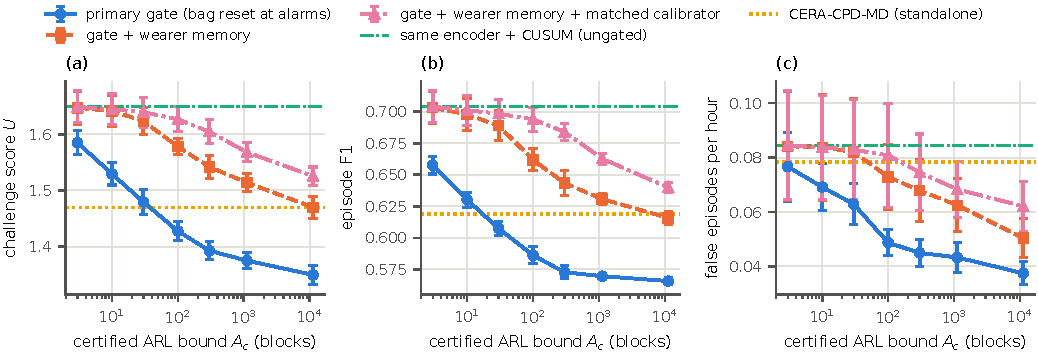
\includegraphics[width=\textwidth]{figures/fig_memory.pdf}
\caption{Price of certification with wearer memory on CPSC2021, showing (a) challenge score, (b) episode F1 and (c) false episodes per hour versus $A_c$ for the primary gate, the memory gate and its matched-calibrator version, with CUSUM and \method{}-MD as references.}
\label{fig:memory}
\end{figure*}

\subsection{Ablation Studies and Computational Cost}
\label{sec:res-ablation}
\label{sec:res-cost}
Decision clipping was essential (Table~\ref{tab:ablation}), because without it the challenge score fell from 1.32 to 1.16 and false episodes rose fivefold. Removing the rhythm stream ($U=1.19$) or the atrial stream ($U=1.25$, with ectopy false alarms tripled) hurt, whereas the learned gate, patient-matched negatives and the contrastive loss made no measurable difference. The warm-up, calibrator, beat-level refinement, fallback and bag restart changed the score by at most 0.01, and the power calibrator raised false episodes on ectopy-rich recordings by 40\%. With seed 0, four-beat blocks lowered the scores of \method{}, CUSUM and smoothing from 1.34, 1.67 and 1.59 to 1.23, 1.58 and 1.57 without recovering short episodes, and sixteen-beat blocks gave 1.34, 1.53 and 1.52, so eight-beat blocks were retained. The encoder has 77\,124 inference parameters and needs $1.8\times10^7$ multiply-accumulate operations per block. Its median single-thread latency on an Intel Core i7-12700 was 3.2\,ms per block and the SR update took 6.2\,$\mu$s, well under 0.1\% of real time for blocks of about 6\,s.

\begin{table}[!htbp]
\centering
\caption{Ablations on CPSC2021 (mean\,$\pm$\,s.d.), with three seeds and the validated threshold for encoder ablations and $\lambda^\star=0.1$/h for detector ablations ($^\ast$). Ectopy FA/h is measured on non-AF recordings with $\ge$1\% ectopic beats. Bold marks the best value.}
\label{tab:ablation}
\footnotesize
\setlength{\tabcolsep}{2.5pt}
\resizebox{\columnwidth}{!}{%
\begin{tabular}{@{}lccccc@{}}
\toprule
Variant & $U$ & Bnd.\ Se$_{\pm1}$ & Ep.\ F1 & FA/h & Ectopy FA/h\\
\midrule
Full model (validated $A$) & 1.31\,$\pm$\,0.02 & 0.8\,$\pm$\,0.2 & 54.8\,$\pm$\,0.6 & \textbf{0.07\,$\pm$\,0.02} & \textbf{0.10\,$\pm$\,0.02}\\
w/o atrial stream & 1.25\,$\pm$\,0.01 & 0.5\,$\pm$\,0.0 & 54.5\,$\pm$\,0.4 & 0.15\,$\pm$\,0.01 & 0.33\,$\pm$\,0.05\\
w/o rhythm stream & 1.19\,$\pm$\,0.01 & 0.6\,$\pm$\,0.0 & 51.6\,$\pm$\,0.7 & 0.11\,$\pm$\,0.01 & 0.12\,$\pm$\,0.01\\
Equal weights (no gate) & 1.32\,$\pm$\,0.02 & 0.9\,$\pm$\,0.1 & 55.0\,$\pm$\,0.6 & 0.08\,$\pm$\,0.01 & 0.13\,$\pm$\,0.02\\
w/o ectopy-nuisance sampling & \textbf{1.35\,$\pm$\,0.03} & 1.1\,$\pm$\,0.4 & \textbf{56.1\,$\pm$\,0.5} & 0.08\,$\pm$\,0.01 & 0.15\,$\pm$\,0.03\\
w/o patient-matched negatives & 1.31\,$\pm$\,0.02 & 0.8\,$\pm$\,0.1 & 55.1\,$\pm$\,0.8 & \textbf{0.07\,$\pm$\,0.01} & 0.11\,$\pm$\,0.02\\
w/o contrastive loss & 1.31\,$\pm$\,0.01 & 0.9\,$\pm$\,0.2 & 55.2\,$\pm$\,0.4 & \textbf{0.07\,$\pm$\,0.01} & 0.11\,$\pm$\,0.04\\
\midrule
Full model, $\lambda^\star=0.1$/h (reference)$^\ast$ & 1.32\,$\pm$\,0.02 & 1.2\,$\pm$\,0.2 & 55.0\,$\pm$\,0.5 & 0.08\,$\pm$\,0.00 & 0.13\,$\pm$\,0.01\\
w/o decision clipping$^\ast$ & 1.16\,$\pm$\,0.02 & 1.1\,$\pm$\,0.3 & 48.4\,$\pm$\,0.3 & 0.38\,$\pm$\,0.02 & 0.52\,$\pm$\,0.03\\
Block-level boundary only$^\ast$ & 1.32\,$\pm$\,0.02 & 0.7\,$\pm$\,0.1 & 55.0\,$\pm$\,0.5 & 0.08\,$\pm$\,0.00 & 0.13\,$\pm$\,0.01\\
Power calibrator, $\kappa=0.3^\ast$ & 1.33\,$\pm$\,0.02 & \textbf{2.1\,$\pm$\,0.2} & 54.9\,$\pm$\,0.5 & 0.09\,$\pm$\,0.01 & 0.18\,$\pm$\,0.02\\
Bag restarted at $\hat k^\ast$ & 1.32\,$\pm$\,0.02 & 1.1\,$\pm$\,0.2 & 55.3\,$\pm$\,0.6 & 0.08\,$\pm$\,0.00 & 0.13\,$\pm$\,0.01\\
Short-episode fallback$^\ast$ & 1.32\,$\pm$\,0.02 & 1.8\,$\pm$\,0.2 & 55.2\,$\pm$\,0.5 & 0.08\,$\pm$\,0.00 & 0.12\,$\pm$\,0.01\\
Warm-up $W=2^\ast$ & 1.32\,$\pm$\,0.02 & 1.2\,$\pm$\,0.2 & 55.0\,$\pm$\,0.5 & 0.08\,$\pm$\,0.00 & 0.13\,$\pm$\,0.01\\
Warm-up $W=8^\ast$ & 1.32\,$\pm$\,0.02 & 1.2\,$\pm$\,0.3 & 55.0\,$\pm$\,0.5 & 0.08\,$\pm$\,0.00 & 0.13\,$\pm$\,0.01\\
\bottomrule
\end{tabular}}
\end{table}


% =====================================================================
\section{Discussion}
\label{sec:discussion}

\subsection{Principal Findings and Interpretation}
The pre-specified hypotheses received mixed support. H1 was not supported, as on the same frozen encoder CUSUM delineated CPSC2021 episodes better than the standalone conformal e-detector across thresholds, seeds and cohorts, and the post hoc wearer memory narrowed but did not reverse this gap. The alarm-control component of H2 was supported where its validity conditions hold, with the bounds met under exchangeability and the nominal budgets on sinus ECG, but not under serial dependence or for very strict thresholds on real ECG. Its ectopy component was not supported robustly and its noise component only weakly. H3 was supported for in-distribution coverage (93 to 97\%), with informative widths only for detectors with small residuals. These conclusions held with causal QRS detection and in EC57 terms.

The secondary analyses lead to a constructive conclusion. The conformal e-detector is weak as a standalone decision rule on short recordings but valuable as a certificate, since gating CUSUM reduced false episodes in cross-validation and on every external cohort and improved the score under heavy noise, at a cost of 0.06 in the clean score. Unlike a tuned threshold, the certificate's guarantee does not depend on how the proposing detector was trained, its strength is an explicit dial (Fig.~\ref{fig:certification}), and it lowered the false episodes of every proposer tested. Wearer memory strengthened both roles. It raised the standalone score by 0.13 to 0.16 and allowed a certificate of $A_c=1121$ to retain the clean accuracy of the weak primary certificate while keeping false episodes under heavy noise at 0.08 per hour (Fig.~\ref{fig:memory}).

Conformal evidence is relative to the wearer's history. A unique new maximum in a bag of $j$ blocks has p-value $\theta_j/j$, and with $n$ pre-change blocks and post-change scores all above them, the expected p-value of the $k$-th post-change block is $k/[2(n+k)]$, so contamination of the reference weakens evidence when the history is short, in line with the suboptimal delay of standard conformal martingales \cite{bhattacharyya2026conformal}. CPSC2021 sits in this unfavourable regime (Section~\ref{sec:res-mech}), and the challenge score, which rewards avoiding false episodes in the many non-AF recordings, drove the validated threshold higher still. During development, two remedies relying on a population-level null, namely seeding the bag with held-out patients' scores and likelihood-ratio e-values normalised on held-out patients, increased false episodes four- to sixty-fold on validation patients. Wearer memory instead stays within the wearer's history. It lengthens the reference for later episodes and recordings but cannot help a new wearer's first episodes or episodes of one or two blocks, consistent with the remaining gap to CUSUM.

\subsection{Patient Adaptation and Clinical Implications}
The mechanism that slows detection also protects against false alarms when scores shift, because a wearer whose non-AF scores rise because of noise or ectopy gradually absorbs them into the reference, whereas a population threshold keeps alarming. This explains the flat false-alarm curves of the standalone detector under electrode-motion noise, which held with R peaks detected from the noisy signal (0.09 vs 0.46 false episodes per hour for CUSUM). A strong certificate suits settings in which review workload takes priority over prompt alarms, and a weak one settings in which delineation accuracy is the priority. With wearer memory, a strong certificate costs much less accuracy, which makes it attractive for long-term monitoring. For a monitoring service, the same-encoder CUSUM produced about one false episode per 12 hours of recording in cross-validation and one per 36 hours on NSRDB. Because these false episodes rarely lasted less than 30\,s, the alarm budget rather than a duration filter governs the review workload. Short challenge events and merged AF/flutter labels must not be interpreted as guideline-level diagnoses, and clinical use requires prospective validation with adjudicated labels and a representative wearable population.

\subsection{Limitations}
\label{sec:limitations}
The false-alarm guarantees of \method{} rest on the exchangeability of the processed scores, which real ECG satisfies only approximately. The pilot, mode switches, resets and episode assembly lie outside the formal guarantee, and no delay optimality or boundary coverage is claimed. The comparison is also limited in scope, since comparator thresholds were tuned for the challenge score, only a subset of published comparators could be reproduced and the overlap-based delay metric can reuse an earlier alarm. Wearer memory requires the stronger condition that a wearer's same-state scores are exchangeable across episodes and recordings. It was developed after the primary results, its resolution-matched calibrator was added after the first CPSC2021 test evaluation of the memory detectors, and the CPSC2021 recordings were processed in record-number order because their chronology is undocumented. Its benefit in prospective multi-day monitoring therefore remains to be confirmed.

The burden intervals provide marginal coverage over exchangeable patients and rely on about 17 calibration patients per fold, so the 90\% quantile lies close to the largest calibration residual and the intervals can be conservative, while coverage on external databases is empirical rather than guaranteed. Finally, the reported latencies were measured on a workstation CPU and exclude preprocessing, peak detection and data transport, so the cost on wearable hardware still has to be established.

% =====================================================================
\section{Conclusion}
\label{sec:conclusion}
\method{} combines a dual-stream ectopy-aware encoder, a decision-clipped conformal e-detector with retrospective localisation and abstention-aware conformal burden intervals. In a patient-disjoint evaluation on 480\,h of CPSC2021 recordings, 2.7\,kh of external and control recordings and 1.1\,kh of noise-stress copies, the standalone conformal detector met its nominal false-alarm budgets on sinus ECG and kept false alarms flat under heavy noise, also with causal QRS detection, but detected episodes later than CUSUM on the same encoder because short recordings leave too little reference history. Used as a certificate on CUSUM proposals, it reduced false alarms on every cohort and improved accuracy under heavy noise. A wearer memory raised the standalone challenge score from 1.31 to 1.47, brought its AFDB episode F1 to the level of CUSUM and allowed a strong certificate to retain the clean accuracy of the weak primary certificate. These results favour rank-based sequential evidence with wearer memory as a certificate on a tuned CUSUM detector, and prospective validation on wearable hardware is the next step.

% =====================================================================
\section*{Acknowledgements}
The authors thank the organisers of CPSC2021 and the creators of the PhysioNet databases used in this study for making their recordings openly available, PhysioNet \cite{goldberger2000physionet} for hosting them, and Dr.\ B.\ R.\ Ambedkar National Institute of Technology Jalandhar for access to its high-performance computing facility.

\section*{Declarations}
\noindent\textbf{Funding.} This work was supported by the Anusandhan National Research Foundation (ANRF), Government of India, under the Prime Minister Early Career Research Grant (PM-ECRG) [Grant/File No. ANRF/\allowbreak ECRG/\allowbreak 2025/\allowbreak 000038/\allowbreak ENS].

\noindent\textbf{Data and code availability.} All recordings analysed in this study are publicly available from PhysioNet \cite{goldberger2000physionet}, namely CPSC2021 \cite{cpsc2021}, AFDB \cite{moody1983afdb}, LTAFDB \cite{petrutiu2007ltafdb}, NSRDB, MIT-BIH Arrhythmia \cite{moody2001mitbih} and NSTDB \cite{moody1984nstdb}. No new data were generated. The complete source code, which reproduces every reported number, table and figure, is publicly available under the MIT licence at \url{https://github.com/guptam1989/CERA-CPD-Atrial-Fibrillation-in-Ambulatory-ECG}. Trained checkpoints and per-record outputs will be deposited in a public archive upon acceptance.

% =====================================================================
% =====================================================================
\bibliographystyle{elsarticle-num}
\bibliography{references}

\end{document}
